\documentclass{llncs}
%
%
\usepackage{amsmath}
\usepackage{amssymb}
%\usepackage{amsthm}
\usepackage[dvips]{graphicx}
\usepackage{makeidx}  % allows for indexgeneration
\usepackage[hyphens]{url}
\usepackage[breaklinks]{hyperref}

% Para activar las notas descomentar la linea siguiente y comentar la segunda
% Para desactivar las notas descomentar la linea segunda y comentar la primera
\usepackage[textwidth=2.2cm]{todonotes}
%\usepackage[disable]{todonotes}


\hyphenation{pro-per-ties}
\hyphenation{ge-ne-ral-ly}
\hyphenation{pre-fe-ren-ces}
\hyphenation{u-sing}
\hyphenation{pu-nish-ment}

\newcommand{\Pow}{\mathcal{P}}
\newcommand{\N}{\operatorname{N}}
\newcommand{\bool}{\operatorname*{\mathcal{B}}}
\newcommand{\Pos}{\operatorname{Pos}}
\newcommand{\Nec}{\operatorname{Nec}}
\newcommand{\Open}{\operatorname{Open}}
\newcommand{\Rp}{\operatorname{Rp}}
\newcommand{\Rn}{\operatorname{Rn}}
\newcommand{\FB}{\operatorname{FB}}
\newcommand{\UC}{\operatorname{UC}}
\newcommand{\T}{\mathcal{T}}
\newcommand{\Rel}{\mathcal{R}}
\newcommand{\C}{\mathcal{C}}
\newcommand{\Boolean}{\mathbb{B}}
\newcommand{\Nat}{\mathbb{N}}
\newcommand{\Q}{\mathbb{Q}}
\newcommand{\R}{\mathbb{R}}
\newcommand{\Z}{\mathbb{Z}}
\newcommand{\Head}{\mathcal{H}}
\newcommand{\Body}{\mathcal{B}}
\newcommand{\Dom}{\mathcal{D}}
\newcommand{\INS}{\mbox{\textbf{insert}}}
\newcommand{\DEL}{\mbox{\textbf{delete}}}
\newcommand{\MOD}{\mbox{\textbf{modify}}}
\newcommand{\REV}{\mbox{\textbf{revise}}}
\newcommand{\AR}{\mbox{\textbf{ AR }}}
\newcommand{\Overlap}{\mbox{\textbf{Overlap}}}
\newcommand{\A}{\mathcal{A}}
\newcommand{\I}{\mathcal{I}}
\newcommand{\M}{\mathcal{M}}
\renewcommand{\Join}{\bowtie}

\begin{document}

\mainmatter              % start of the contributions
%
\title{A relational algebra for temporal databases}
%\title{Introducing valid time in bipolar database querying}
%
%\titlerunning{A Fuzzy Valid-Time Model}  % abbreviated title (for running head)
%                                     also used for the TOC unless
%                                     \toctitle is used
%
\author{Jose Enrique Pons\inst{1} \and Christophe Billiet\inst{2} \and Guy De Tr\'e\inst{2} \and Olga Pons Capote\inst{1} }

%
%\authorrunning{Ivar Ekeland et al.} % abbreviated author list (for running head)
%
%%%% list of authors for the TOC (use if author list has to be modified)
%\tocauthor{Ivar Ekeland, Roger Temam, Jeffrey Dean, David Grove,
%Craig Chambers, Kim B. Bruce, and Elisa Bertino}
%
\institute{Department of Computer Science and Artificial Intelligence \\
University of Granada \\
C/Periodista Daniel Saucedo Aranda s/n E-18071 (Granada-Spain) \\
\email{jpons,opc@decsai.ugr.es}\\ 
%WWW home page:
%\texttt{http://users/\homedir iekeland/web/welcome.html}
%\and
%Universit\'{e} de Paris-Sud,
%Laboratoire d'Analyse Num\'{e}rique, B\^{a}timent 425,\\
%F-91405 Orsay Cedex, France
\and 
Department of Telecommunications and Information Processing,\\
Ghent University,\\
Sint-Pietersnieuwstraat 41, B-9000 Ghent, Belgium\\
\email{Christophe.Billiet,Guy.DeTre@UGent.be}
}

\maketitle              % typeset the title of the contribution

\begin{abstract}

%%%%%%%%%%%%%%%%%%%%%%%%%
%
% ABSTRACT
%
%%%%%%%%%%%%%%%%%%%%%%%%
In reality, some objects or concepts have properties with a time-variant or time-related nature. Modelling these kinds of objects or concepts in a (relational) database schema is possible, but time-variant and time-related attributes have an impact on the consistency of the entire database. Therefore, temporal database models have been proposed to deal with this. Time itself can be at the source of imprecision, vagueness and uncertainty, since existing time measuring devices are inherently imperfect. Accordingly, human beings manage time using temporal indications and temporal notions, which may contain imprecision, vagueness and uncertainty. However, the imperfection in human-used temporal indications is supported by human interpretation, whereas information systems need support for this. Several proposals for dealing with such imperfections when modelling temporal aspects exist. Some of these proposals transform the temporal expression into a compact representation. Other proposals consider the temporal indications in the used temporal expressions to be the source of imperfection. 
In this work we present a novel model to deal with imperfections in valid-time databases. Next to that, the data manipulation language, \emph{DML} is defined and implemented.

\end{abstract}

%
\section{Introduction}

%
%%%%%%%%%%%%%%%%%%%%%%%%%%%%%%%%%%%%%%%%%%%%%%%%%%%%%%%%%%%%%%%%%%%%%%
%
% Introduction
%
%%%%%%%%%%%%%%%%%%%%%%%%%%%%%%%%%%%%%%%%%%%%%%%%%%%%%%%%%%%%%%%%%%%%%%

The concept of time is very complex to handle and interpret~\cite{Klein1994,Shackle1961}, though it is very natural and omnipresent in real world data. As information systems attempt the modelling of natural objects, concepts or processes, they often require modelling temporal aspects or concepts. Thus, several proposals have arisen to obtain theoretical models that allow the modelling or representation of time~\cite{Bolour1982,VanderCruyssen1997}.

A very specific type of information systems are database systems. A database contains data representing real objects or concepts. In real world, some aspects or properties of objects are time-variant or time-related. e.g., the moment of a bank transaction and the status of an employee in a company, are time-related and time-variant notions, respectively.
A temporal database schema is a database schema that models objects with time-related or time-variant properties. However, the modelling of temporal aspects has a direct impact on the consistency of the temporal database, because the temporal nature of these aspects imposes extra integrity constraints and suitable ways of interactive with the human user. 

For example, let us consider a hospital database containing data about the state of the patients in a given hospital. Two dates are stored: the date when the patient arrives to and leaves from the hospital. It is clear that a patient cannot leave the hospital if he or she has not arrived. Without further cautions, a hospital employee could insert a patient who is already in the hospital. A temporal database model will typically constrain record insertion and prevent similar modelling inconsistencies.

A lot of research concerns temporal database models and their approaches to the modelling of time. The first efforts were towards the representation of historical information related to objects represented by records in a database~\cite{Clifford1985}. Some proposals tried to extend the Entity Relationship Model~\cite{Klopprogge1983}, without impact on any database standards like SQL~\cite{Sarda1990}.

Notably, in 1994, ``A Consensus Glossary of Temporal Database Concepts'' was published~\cite{Dyreson1994}. For this publication, 44 temporal database researchers, among them, some of the main researchers in this field, cooperated to reach a consensus on the nature and definitions of some of the main temporal database concepts and terminology. This glossary was updated in 1998~\cite{Dyreson1998}.


% %From time in general to time in information systems
% In real world, some aspects or properties of objects, concepts or processes are time-variant or time-related. For example, the moment of a bank transaction is traditionally a point in time and thus a time-related notion, the function of an employee in a company can change through recorded history and is thus time-variant.  As information systems often attempt the modelling of natural objects, concepts or processes, they often require modelling temporal aspects or concepts. Thus, several proposals have been concerned with obtaining theoretical models that allow the modelling or representation of time~\cite{Bolour1982},~\cite{VanderCruyssen1997}.

% %From time in information systems to time in temporal databases
% Time is a complex concept, which makes modelling time in database systems complex too. A \emph{temporal database} is a database that deals with certain time-related aspects in its schema: a \emph{temporal database schema}~\cite{Dyreson1994} is a database schema that models entities (and interactions or relationships between entities) with time-related or time-variant properties. However, the modelling of temporal properties or aspects has a direct impact on the consistency of the resulting temporal database, because the temporal nature of these aspects or properties imposes extra integrity constraints. An example. Consider a relation in a relational library database, representing the physical absence (or presence) of books in the library. Every physical book is represented by a unique identifier. Every record in the relation contains such an identifier, a date on which the corresponding book was loaned and a date on which it was subsequently returned (if it was returned). As such, every record represents a period of time during which the physical book corresponding with the identifier is loand to a library customer. Without further precautions, a library employee could add several records with the same book identifier, different `loaned'-dates and no `returned'-dates. This group of records would represent the same physical book being loaned several times on different dates and never returned, which is of course impossible. A temporal database model will typically constrain record insertion and prevent similar modelling inconsistencies.

An interesting issue in temporal modelling concerns relationships between temporal notions. In this sense, Allen~\cite{Allen1983} studied temporal relationships between time intervals (and as a special case time points). Among others, the querying of temporal databases has greatly profited from these temporal relationships, because they allowed more powerful user-specified temporal query demands, by allowing to express more complex relationships between the temporal notions in the temporal expressions in the query. For example, a query like `who were the department heads when Thomas worked for the institution' can be evaluated using operators similar to Allen's ones.

Humans handle temporal information using certain temporal notions like time intervals or time points~\cite{Dyreson1994}, and they often have to deal with imperfections like imprecision, vagueness, uncertainty or inconsistencies possibly contained in the descriptions of these temporal notions. These possible imperfections in descriptions of temporal notions determine an important issue in temporal modelling. Consider as an example the description of the temporal notion in a sentence like `The Belfry of Bruges was finished between 01/01/1201 A.D. and 31/12/1300 A.D.'. These sentence contains imperfection because of the uncertainty in the used time-related expression. It is known that the building was finished on a single day, but this day is not precisely known.

To allow information systems to cope with these and similar data imperfections, many approaches adopt fuzzy sets~\cite{Zadeh1965} for the representation and management of temporal information~\cite{Mitra1994,Nagypal2003,Billiet2011,Dubois2003}. The temporal relationships studied by Allen were fuzzified by several authors~\cite{Ohlbach2004,Nagypal2003,Schockaert2008}.   Garrido et al. ~\cite{Garrido2009} presented a compact representation for the time and defined different relationships among time intervals by using a combination of regular fuzzy comparisons. Also ~\cite{Garrido2009,Pons2011} studied uncertainty in temporal expressions concerning time intervals. Other approaches, like~\cite{Qiang2009}, use rough sets~\cite{Pawlak1995} to represent time intervals.

%Now introducing imperfections in representations of time...
% Humans handle temporal information using certain temporal notions like specific time intervals or instants~\cite{Dyreson1994} and they often have to deal with imperfections like imprecisions, vaguenesses, uncertainties or inconsistencies possibly contained in (the descriptions of) these temporal notions. Among many others, these possible imperfections in (descriptions of) temporal notions determine an important issue in temporal modelling. As an example, consider the temporal notion described in a sentence like `The Belfry of Bruges was finished on a day somewhere between 01/01/1201 A.D. and 31/12/1300 A.D.'. The description of the temporal notion reads `a day somewhere between 01/01/1201 A.D. and 31/12/1300 A.D.'. This temporal notion thus contains imperfection in the form of the uncertainty about the exact day the last stone of the building was laid: it is known that the building was finished on a single day, but it is not known which day this was. To allow information systems to cope with these and similar temporal data imperfections, many approaches adopt fuzzy sets~\cite{Zadeh1965} and/or fuzzy logic to model temporal information~\cite{Mitra1994},~\cite{Nagypal2003},~\cite{Billiet2011},~\cite{Dubois2003}. 

In addition to temporal modelling, some attention has been paid to temporal reasoning~\cite{Allen1983}. Although temporal reasoning is not discussed in this paper, it should be noted that, among others, Dubois and Prade et al.~\cite{Dubois2003,DuBois1989} have dealt with fuzziness and uncertainty in temporal reasoning.

The present work defines and implement a model for properly represent and manage uncertainty in valid-time specification in a relational database. Our work is focused on both the proposal of an appropriate formal framework to suitably manage time in databases and the implementation of an DML that allows to the user the transparent use of this proposal. None of the previous research offer a database model to accomplish this task.

This way together with the theoretical model, we also present and explain the main operations of the manipulation language for a temporal database which stores the valid-time periods of the objects affected by imprecision. The rest of the work is organized as follows. Section \ref{sec:prelim} presents some background concepts about both possibility theory and temporal databases. In section \ref{sec:time-rep} the representation of the valid-time intervals in the database is explained. Section \ref{sec:temporal-model} explains the main concepts of the temporal Data Manipulation Language (DML) and its implementation. Finally, Section \ref{sec:conclusions} presents the conclusions and some guidelines for future research work.


% 
% 
% %From information systems in general to database systems in particular:
% Generally, \emph{information systems} model the structure and behavior of real objects, concepts or processes. A specific type of information systems are \emph{database systems}, which are computer systems designed to manage \emph{databases}. A database is basically a collection of (persistent) data. These (typically atomic) data represent real objects or concepts. In the context of database design, such objects or concepts are typically called \emph{entities} and a collection of similar entities is typically modelled by an \emph{entitytype}, which is basically a combination of a name and a list of \emph{attributes}, which describe properties of the entities. Typically, in an early stage of the database development process, the structures of and interactions or relationships between used entities are modelled in a \emph{design schema}, following some design model. A database thus contains (typically atomic) data. Each (atomic) part of these data is a result value of a measurement of a property of an entity or a description of a property of an entity and will correspond to the attribute of the entity's entitytype, which describes the property.
% 
% %From database models in general to the relational model in particular:
% The structure and behavior of a database, along with some integrity and security restrictions, is dictated by a \emph{database model}. A database model is basically a collection of instructions and regulations, used to (logically) describe the structure and behavior of a database, along with some integrity and security restrictions. Applying a database model to a concrete design schema results in a \emph{database schema}, which models the logical structure and behavior of a database. Several different database models exist, but the most popular is the \emph{relational database model}~\cite{Codd:1970:RMD:362384.362685}. Following the relational database model, entitytypes are modelled as \emph{relations}, which comprise a name and a list of attributes, modelling the entitytype's attributes.
% 
% %From time in general to time in information systems
% In reality, some aspects or properties of objects, concepts or processes are time-variant or time-related. For example, the moment of a bank transaction is traditionally a moment in time and thus a time-related notion, the function of an employee in a company can change through recorded history and is thus time-variant. The concept of time itself is very complex to handle and interpret~\cite{Klein1994},~\cite{Shackle1961}, though it is very natural and omnipresent. As information systems often attempt the modelling of natural objects, concepts or processes, they often require modelling temporal aspects or concepts. Thus, several proposals have been concerned with obtaining theoretical models that allow the modelling or representation of time~\cite{Bolour1982},~\cite{VanderCruyssen1997}.
% 
% %From time in information systems to time in temporal databases
% Time is a complex concept, which makes modelling time in database systems complex too. A \emph{temporal database} is a database that deals with certain time-related aspects in its schema: a \emph{temporal database schema}~\cite{Dyreson1994} is a database schema that models entities (and interactions or relationships between entities) with time-related or time-variant properties. However, the modelling of temporal properties or aspects has a direct impact on the consistency of the resulting temporal database, because the temporal nature of these aspects or properties imposes extra integrity constraints. An example. Consider a relation in a relational library database, representing the physical absence (or presence) of books in the library. Every physical book is represented by a unique identifier. Every record in the relation contains such an identifier, a date on which the corresponding book was loaned and a date on which it was subsequently returned (if it was returned). As such, every record represents a period of time during which the physical book corresponding with the identifier is loand to a library customer. Without further precautions, a library employee could add several records with the same book identifier, different `loaned'-dates and no `returned'-dates. This group of records would represent the same physical book being loaned several times on different dates and never returned, which is of course impossible. A temporal database model will typically constrain record insertion and prevent similar modelling inconsistencies.
% 
% %Research about temporal databases
% A lot of research concerns temporal database models and their approaches to the modelling of time. Some of the first proposals concerned the representation of historical information related to entities~\cite{Clifford1985}. Some proposals tried to extend the Entity Relationship Model~\cite{Klopprogge1983}, without impact on any database standards like SQL~\cite{Sarda1990}. Notably, in 1994, `A Consensus Glossary of Temporal Database Concepts' was published~\cite{Dyreson1994}. For this publication, 44 temporal database researchers, among which some of the main researchers in this field, cooperated to reach a consensus on the nature and definitions of some of the main temporal database concepts and their terminology. This glossary was subsequently updated in 1998~\cite{Dyreson1998}. In the presented work, the concepts and terminology from this glossary are used and followed.
% 
% %Research about temporal relationships
% An interesting issue in temporal modelling concerns the relationships between temporal notions. Notably, Allen~\cite{Allen1983} studied temporal relationships between time intervals~\cite{Dyreson1994} (and, as a special case, instants~\cite{Dyreson1994}). Among others, the querying of temporal databases has greatly profited from these temporal relationships, because they allow for richer and more complex user-specified temporal query demands, by allowing to express more complex relationships between the temporal notions in the temporal expressions in the query and the temporal indications in the database. For example, given a relation representing who was department head of an institution during which time intervals, a query like `Who were the department heads during the time intervals when Thomas worked for the institution?' can be evaluated using similar relationships. %TODO: CHECK THIS LAST SENTENCE
% 
% %Now introducing imperfections in representations of time...
% Humans handle temporal information using certain temporal notions like specific time intervals or instants~\cite{Dyreson1994} and they often have to deal with imperfections like imprecisions, vaguenesses, uncertainties or inconsistencies possibly contained in (the descriptions of) these temporal notions. Among many others, these possible imperfections in (descriptions of) temporal notions determine an important issue in temporal modelling. As an example, consider the temporal notion described in a sentence like `The Belfry of Bruges was finished on a day somewhere between 01/01/1201 A.D. and 31/12/1300 A.D.'. The description of the temporal notion reads `a day somewhere between 01/01/1201 A.D. and 31/12/1300 A.D.'. This temporal notion thus contains imperfection in the form of the uncertainty about the exact day the last stone of the building was laid: it is known that the building was finished on a single day, but it is not known which day this was. To allow information systems to cope with these and similar temporal data imperfections, many approaches adopt fuzzy sets~\cite{Zadeh1965} and/or fuzzy logic to model temporal information~\cite{Mitra1994},~\cite{Nagypal2003},~\cite{Billiet2011},~\cite{Dubois2003}. 
% 
% %Now introducing imperfections in temporal relationships
% The temporal relationships studied by Allen were fuzzified by several authors~\cite{Ohlbach2004},~\cite{Nagypal2003},~\cite{Schockaert2008}. Garrido et al. ~\cite{Garrido2009} present different temporal operators, defined by a combination of fuzzy comparisons. Also,~\cite{Garrido2009},~\cite{Pons2011} studied uncertainty in the context of time intervals. Other approaches, like~\cite{Qiang2009}, use rough sets~\cite{Pawlak1995} to represent time intervals.
% 
% %Imperfections in temporal reasoning
% Next to temporal modelling, some attention has gone to temporal reasoning~\cite{Allen1983}. Although the focus of this paper is temporal modelling, it should be noted that, among others, Dubois and Prade et al.~\cite{Dubois2003},~\cite{DuBois1989} have dealt with fuzziness and uncertainty in temporal reasoning.
% 
% %Overview of this work
% %Include: what is the paper about? (situation and explanation of the problem we will solve and situation of our solution (we use constraints...))
% %Include: how does the solution work? (short summary of how the solution will solve the problem/attend to the problem)
% %Include: What exactly will be presented
% %In all of these: stress every single innovative/novel point of the presented work!
% %TODO: build the overview when the paper is finished
% 
% The aim of this work is to present and explain the main operations of the manipulation language for a temporal database which stores the valid-time periods of the objects with uncertainty. The rest of the work is organized as follows. Section \ref{sec:prelim} presents some background concepts about both possibility theory and temporal databases. In section \ref{sec:time-rep} the representation of the valid-time intervals in the database is explained. Section \ref{sec:temporal-model} explains the main concepts and behaviour of the temporal model. The Data Manipulation Language (DML) is described and implemented. Finally in Section \ref{sec:conclusions} presents the conclusions and some possibilities for future research work.
% 


%
\section{\label{sec:preliminaries}Preliminaries}
The basics on possibility theory is introduced within the first subsection. Then, some background concepts about temporal databases are introduced. Finally, the representation of imperfect temporal intervals is explained.
\subsection{\label{subsec:possibilistic-variables}Possibilistic Variables}
Possibilistic variables rely on possibility theory \cite{Dubois1988a}. A \emph{possibilistic variable} is defined as follows \cite{Pons2011}.

\begin{definition}
A possibilistic variable $X$ over a universe $U$ is defined as a variable taking exactly one value in $U$, but for which this value is (partially) unknown. Its possibility distribution $\pi_X$ on $U$ models the available knowledge about the value that $X$ takes: for each $u\in U$, $\pi_X(u)$ represents the possibility that $X$ takes the value $u$. In this work, this possibility is interpreted as a measure of how plausible it is that $X$ takes the value $u$, given (partial) knowledge about the value $X$ takes.
\end{definition}

The exact value a possibilistic variable takes, which is (partially) unknown, is called an \emph{ill-known value} in this work \cite{Dubois1988a}.

When a possibilistic variable is defined on the powerset $\Pow(R)$ of some universe $R$, the unique value the variable takes will be a crisp set and its possibility distribution on the powerset $\Pow(R)$ will describe the possibility of each crisp subset of $R$ to be the value the variable takes. This exact value (a crisp set) the variable takes, is now called an \emph{ill-known set} \cite{Dubois1988a}.


A specific application of possibilistic variables is obtained when the universe under consideration is the set of Boolean values $\mathbb{B}$ = $\{T,F\}$. Indeed, any Boolean proposition $p$ takes just one value in $\mathbb{B}$. If the knowledge about which value this proposition $p$ will take is given by a possibility distribution $\pi_p$, the proposition can be seen as a possibilistic variable. As the interest lies with the case where the proposition holds, the possibility and necessity that $p$ = $T$ (the proposition holds) demand most attention. This possibility and necessity is noted here as:
\begin{align}
\text{Possibility that $p$ = $T$ (p holds):} \hspace{50pt} & Pos(p) = \pi_p(T) \label{propholdsposs} \\
\text{Necessity that $p$ = $T$ (p holds):} \hspace{50pt} & Nec(p) = 1-\pi_p(F) \label{propholdsnecc}
\end{align}

This work will deal with ill-known intervals. These are ill-known sets, defined and represented via a start and end point, which will be ill-known values. The elements of the set are the values between the start and end point. A closed ill-known interval with start point defined by possibilistic variable $X$ and end point by possibilistic variable $Y$ is noted here $\left[X, Y\right]$. The correspondences and transitions between the representations of ill-known sets, between the representations of ill-known intervals and between the representations of an ill-known set and an ill-known interval are part of the authors current research.

\subsection{\label{subsec:fuzzy-numbers}Fuzzy Numbers and Fuzzy Intervals}
Among others, Dubois and Prade~\cite{Dubois1983} use fuzzy sets \cite{Zadeh1965} to define a \emph{fuzzy interval}:
\begin{definition}
A fuzzy interval is a fuzzy set $M$, defined by a membership function $\mu_{M}$, on the set of real numbers $\mathbb{R}$ such that:
\begin{eqnarray}
\mu_{M} : & \!\!\!\!\!\!\!\!\!\!\!\!\!\!\!\!\!\!\!\!\!\!\!\!\!\!\!\!\!\!\!\!\!\!\!\!\!\!\!\!\!\!\!\!\!\!\!\!\!\! \mathbb{R} \rightarrow \left[0,1\right] \nonumber \\ 
\forall (u,v)\in\mathbb{R}^2: \forall w \in [u,v]:&\mu_M(w) \geq\min(\mu_M(u),\mu_M(v))  \\
\exists m \in \mathbb{R} : & \!\!\!\!\!\!\!\!\!\!\!\!\!\!\!\!\!\!\!\!\!\!\!\!\!\!\!\!\!\!\!\!\!\!\!\!\!\!\!\!\!\!\!\!\!\!\!\! \mu_M(m)=1 
\end{eqnarray}
\end{definition}
If this modal value $m$ is unique, then $M$ is referred to as a \emph{fuzzy number}. In other words, if the core of a fuzzy interval is a singleton, it is referred to as a fuzzy number.

The most convenient form of the membership function of a fuzzy number is a triangular form. It can be shown that such a membership function $\mu_M$ for a fuzzy number $M$ is convex and normalized. Three real values, denoted by $a$, $b$ and $D$, suffice to represent a triangular membership function of a fuzzy number and in this work, a fuzzy number defined as such will be noted as $\left[D, a, b \right]$. Here:
\begin{itemize}
\item
$D$ denotes the single value in the core of $M$
\item
$D-a$ is then $\inf \{u \in \mathbb{R} : \mu_{M}(u) > 0\}$
\item
$D+b$ is then $\sup \{u \in \mathbb{R} : \mu_{M}(u) > 0\}$
\end{itemize}

\subsection{Interval Evaluation by Ill-known Constraints}
The problem of interval evaluation is more generally explained in \cite{Pons2011}: the need exists to know if all points in a crisp interval $I$ reside between the boundaries of an ill-known interval $\left[ X , Y \right]$. In \cite{Pons2011}, the notion of an \emph{ill-known constraint} is introduced:

\begin{definition}
Given a universe $U$, an ill-known constraint $C$ on a set $A \subseteq U$ is specified by means of a binary relation $R \subseteq U^{2}$ and a fixed, ill-known value denoted by its possibilistic variable $V$ over $U$, i.e.:
\begin{align}
C \triangleq (R,V)
\end{align}
Set $A$ now satisfies the constraint if and only if:
\begin{align}
\forall a \in A : (a,V) \in R
\end{align}
\end{definition}

An example of an ill-known constraint is $C_{ex} \triangleq (<, X)$. Some set $A$ then satisfies $C_{ex}$ if $\forall a \in A : a < X$, given possibilistic variable $X$.

The satisfaction of a constraint $C \triangleq (R,V)$ by a set $A$ is basically still a Boolean matter, but due to the uncertainty about the ill-known value $V$, it can be uncertain whether $C$ is satisfied by $A$ or not \cite{Pons2011}. In fact, this satisfaction now behaves as a proposition. Based on the possibility distribution $\pi_{V}$ of $V$, the possibility and necessity that $A$ satisfies $C$ can be found. This proposition can thus be seen as a possibilistic variable on $\mathbb{B}$. The required possibility and necessity are:

\vspace{-10pt}

\begin{align}
\Pos(A\text{ satisfies }C) & = \min_{a \in A}\left(\sup_{(a,w) \in R}\pi_{V}(w)\right) \label{ill-known-pos}\\
\Nec(A\text{ satisfies }C) & = \min_{a \in A}\left(\inf_{(a,w) \notin R} 1-\pi_{V}(w)\right) \label{ill-known-nec}
\end{align}

Now, e.g., to check if crisp interval $I = \left[j, k\right]$ is included in $\left[X, Y\right]$, 2 ill-known constraints are constructed:

\vspace{-10pt}

\begin{eqnarray}
C_1 & \triangleq\left(\geq,X\right)\\
C_2 & \triangleq\left(\leq,Y\right)
\end{eqnarray}

To calculate the possibility and necessity concerning a conjunction of constraints, the $\min$ operator can be used. The possibility and necessity of $I$ being included in $\left[X, Y\right]$ are now: 

\vspace{-10pt}

\begin{align}
\label{eq:interval-pos}
\Pos(I\text{ satisfies }C_1\ and\ C_2) & = \min_{a \in I}\left(\sup_{a \geq w}\pi_{X}(w),\sup_{a \leq v}\pi_{Y}(v)\right)\\
\label{eq:interval-nec}
\Nec(I\text{ satisfies }C_1\ and\ C_2) & = \min_{a \in I}\left(\inf_{a < w} 1-\pi_{X}(w),\inf_{a > v} 1-\pi_{Y}(v)\right).
\end{align}
\subsection{Time in databases}
%
%%%%%%%%%%%%%%%%%%%%%%%%%%%%%%%%%%%%%%%%%%%%%%%%%%%%%%%%%%%%%%%%%%%%%%%%%
%
% Time
%
%%%%%%%%%%%%%%%%%%%%%%%%%%%%%%%%%%%%%%%%%%%%%%%%%%%%%%%%%%%%%%%%%%%%%%%%%
The concept of time has been studied in databases for a long time. A true standard for adding temporal aspects to relational databases does not exist, but there is a consensus in the literature \cite{Dyreson1994} on what is called a \emph{temporal database}: a temporal database is a database dealing with some aspects of time in its schema.
In a temporal DBMS, a \textbf{chronon} is the shortest duration of time supported by the system. In temporal databases, some temporal attributes can be managed without treating the attribute differently from non-temporal attributes. The time described by such an attribute is called \textbf{user defined time} (\emph{UDT}). In addition to UDT, the following types of time can be discerned in a temporal database, all of which are handled exceptionally by the DBMS:

\begin{itemize}
	\item
	\textbf{Transaction time} (\emph{TT}) \cite{L.Rowe1987},\cite{Jensen1991a} denotes the time when the fact (object) is stored in the database. It is usually append-only: as the past can not be changed, TT can not be changed neither. Furthermore, at the moment of insertion, a TT can be neither in the past nor in the future.
	\item
	\textbf{Valid time} (\emph{VT}) \cite{Jensen1994},\cite{Sarda1990} denotes the time when the fact (object) is true in the modelled reality. A fuzzy extension has been proposed by \cite{Garrido2009}. 
%	\item
%	User defined time: It is an uninterpreted attribute. The domain is date/time. The query language has no special support for it.
	\item
	\textbf{Decision time} (\emph{DT}, proposed in \cite{Nascimento1995}) denotes the time when an event was decided to happen. 
	\end{itemize}
	
	E.g., consider a database containing employee contract descriptions. The time when the employee's contract is valid, represented by an interval, is VT. The time when the employee's contract is stored in the database is the TT. The time when the decision for hiring this employee was made is the DT.

% is a non-decomposable unit of time.  it  There are two ways to represent a chronon: as a point or as an interval \cite{655777}.

When working with these time concepts, the Data Manipulation Language (\emph{DML}, which is part of the standard database querying language SQL) is extended to deal with possible temporal inconsistencies within the data and to handle more complex (temporal) queries. 
%Next to these concepts, also \textbf{user defined time} (\emph{UDT}) is discerned. UDT is an uninterpreted attribute in the date/time domain. This means that the attribute uses the date/time domain, but the database model does not treat the attribute differently from non-temporal attributes.
Depending on the time managed, a database is classified as either a \textbf{Valid Time Database} (\emph{VTDB}), a \textbf{Transaction Time Database} (\emph{TTDB}), a \textbf{bi-temporal database} (both valid and transaction time are managed) or a \textbf{tri-temporal database} (valid time, transaction time and decision time are managed).

%\subsection{Temporal Elements}
%%	
%	In order to define a temporal database model, some basic elements should be defined \cite{Dyreson1994}:
%	\begin{itemize}
%	\item A	\textbf{chronon} is a non-decomposable unit of time. In a temporal DBMS, it is the shortest duration of time supported by the system. There are two ways to represent a chronon: as a point or as an interval \cite{655777}.
%	\item
%	\emph{Event}: An instant of time. Usually, an event is said to be occur during time $t$ if it occurs during the chronon represented by $t$.
%	\item
%	\emph{Interval}: The time between two events. The representation is very often a set of contiguous chronons.
	%\item
	%\emph{Span}: A directed duration of time. A duration is an amount of time with known  lenght but no specific starting or ending chronons. The span can be either positive, denoting a forward motion of time or negative, denoting a backward motion of time.
%	\item A	\textbf{timestamp} is a time value associated with some object in the database.	
	
%	\item The	\textbf{lifespan} (of a database object)is the time over which it is defined. The lifespan of a valid time object denotes the time when the corresponding object exists. The lifespan of a transaction time object is the value of the timestamp.
	
	
	
	
	
%	Depending on the type of time the meaning is different:
%		\begin{itemize}
%		\item
%		Lifespan of a valid time object: Refers the time when the corresponding object exists.	
%		\item
%		Lifespan of a transaction time object: The transaction time of a database object refers when the object is stored in the database. The lifespan is the value of the timestamp.		
%		\end{itemize}
%	\end{itemize}
	
%	In the temporal database thesaurus, \emph{'Snapshot'} is the word for non-temporal matters. As a temporal database is a generalization for relational databases, an \emph{snapshot database} is a relational database. Furthermore, a \emph{snapshot relation} is a relation incorporating neither valid nor transaction time.

%\subsection{Main issues when dealing with time}
%Among others, the following problems are present when dealing with time in a database:

%	\begin{itemize}	
%	\item \textbf{Granularity} denotes a partition on the set of chronons. The conversion between several granularities is studied in \cite{Lin97efficientconversion}. Granularity is the base of the temporal model in \cite{Cru97}. An object-oriented implementation is in \cite{624013}.
%	\item	To ensure \textbf{consistency}, temporal databases usually redefine the primary key of a relation. The new primary key takes into account the presence of the time. In order to keep the consistency, the DML is re-defined. For example, in a VTDB, the temporal update sentence is usually composed by an update sentence (closing the old row) plus an insert sentence (creating the new row).
%	\end{itemize}
%Guy's suggestion: instead of imprecision, use imperfection which is more general.
% \subsubsection{Imperfection and time}
% Representing imprecision and its semantics when dealing with time has been studied for a long time. Several proposals for representing and computing imprecise time indications can be found in \cite{DeCaluwe1997} and \cite{DeTre1997a}. Also, the changes between several granularities can be seen as a source of imprecision \cite{Devos1998}.
% 
% In the proposal section we will consider two kinds of imprecision:
% \begin{itemize}
% \item \textbf{Uncertainty in the database} denotes the uncertainty that arises when the knowledge about the temporal data in the database is uncertain. E.g., a database record shows that \emph{`The car is in the garage around April.'}
%  \item \textbf{Imprecision in the query specification} denotes the imprecision in the specification of temporal criteria by the user, when querying. E.g., \emph{`The user wants to obtain a car which is red and which is in the garage around April.'}
% \end{itemize}

\subsubsection{Representation}
Several proposals for representing uncertain time in a database exist. Some proposals work with rough sets \cite{Qiang2009}, other proposals rely on possibility distributions for representing uncertainty in time \cite{Garrido2009}, \cite{Galindo2001}. In order to compare temporal possibility distributions, extensions of the classical Allen's operators \cite{Allen1983} are defined in \cite{Ohlbach2004} and \cite{Nagypal2003}. In the proposal section, we will follow the representation by means of possibility distributions, in order to work with both satisfaction and dissatisfaction degrees. Also, in order to work properly with fuzzy operators, the underlying domain should be numeric. In this paper, the representation for the dates will follow the Julian Day Number (JDN) representation \cite{Husfeld1996}.

If the starting points and/or the end points of the interval representing the time are not known precisely, it is easy to fuzzify them, using, e.g., two triangular possibility distributions.
\begin{definition}
A \textbf{Fuzzy Validity Period} (\emph{FVP}) is defined as a fuzzy time interval specifying when an object is valid. A fuzzy time interval is then the fuzzification of a crisp time interval. Several options to transform possibility distributions corresponding to the fuzzy starting point and the fuzzy end point into one consistent FVP exist \cite{Garrido2009}, e.g (Fig. \ref{fig:fuzzy-validity-period}):
\begin{itemize}
\item The \textbf{convex hull} approach is the most intuitive approach. The resulting FVP is the convex hull of the union of both fuzzy sets.
\item The \textbf{uncertainty preserving} approach is less intuitive but more realistic. The amount of uncertainty is maintained at the edges of the possibility distribution representing the FVP \cite{Garrido2009}.
\end{itemize}
\end{definition}


\begin{definition}
A \emph{Possibilistic Valid-time Period} is an ill-known interval in time, which models a time period during which an object in a certain state is valid.
\end{definition}

Because a PVP is an ill-known interval, it allows modelling the uncertainty about the start and/or end point of a time interval (and thus about the time interval itself) if such uncertainty exists. The interpretation is \emph{disjunctive}: the PVP represents exactly one valid-time interval, but precisely \emph{which} interval is represented, is (partially) unknown. In the presented model, only PVPs are considered of which the possibility distributions of the possibilistic variables defining the start and end point of the ill-known interval have exactly the same characteristics as the membership functions of fuzzy numbers. A perfectly known start or end point can then be modelled by such an ill-known value defined by a possibilistic variable $P$ for which $\exists ! x : \mu_{P}(x) > 0$.

As mentioned in \cite{Pons2011}, this approach differs from the one where a valid-time period is represented by one fuzzy set. Such a fuzzy set is seen as a possibility distribution on $\mathbb{R}$ and thus defines just one ill-known value. However, in the presented approach, a time period is modelled using an ill-known set, which is defined by a possibility distribution on $\Pow(\mathbb{R})$.


%%%%%%
% FUZZY VALIDITY PERIOD
%%%%%%
\begin{figure}[h!]
  \centering
  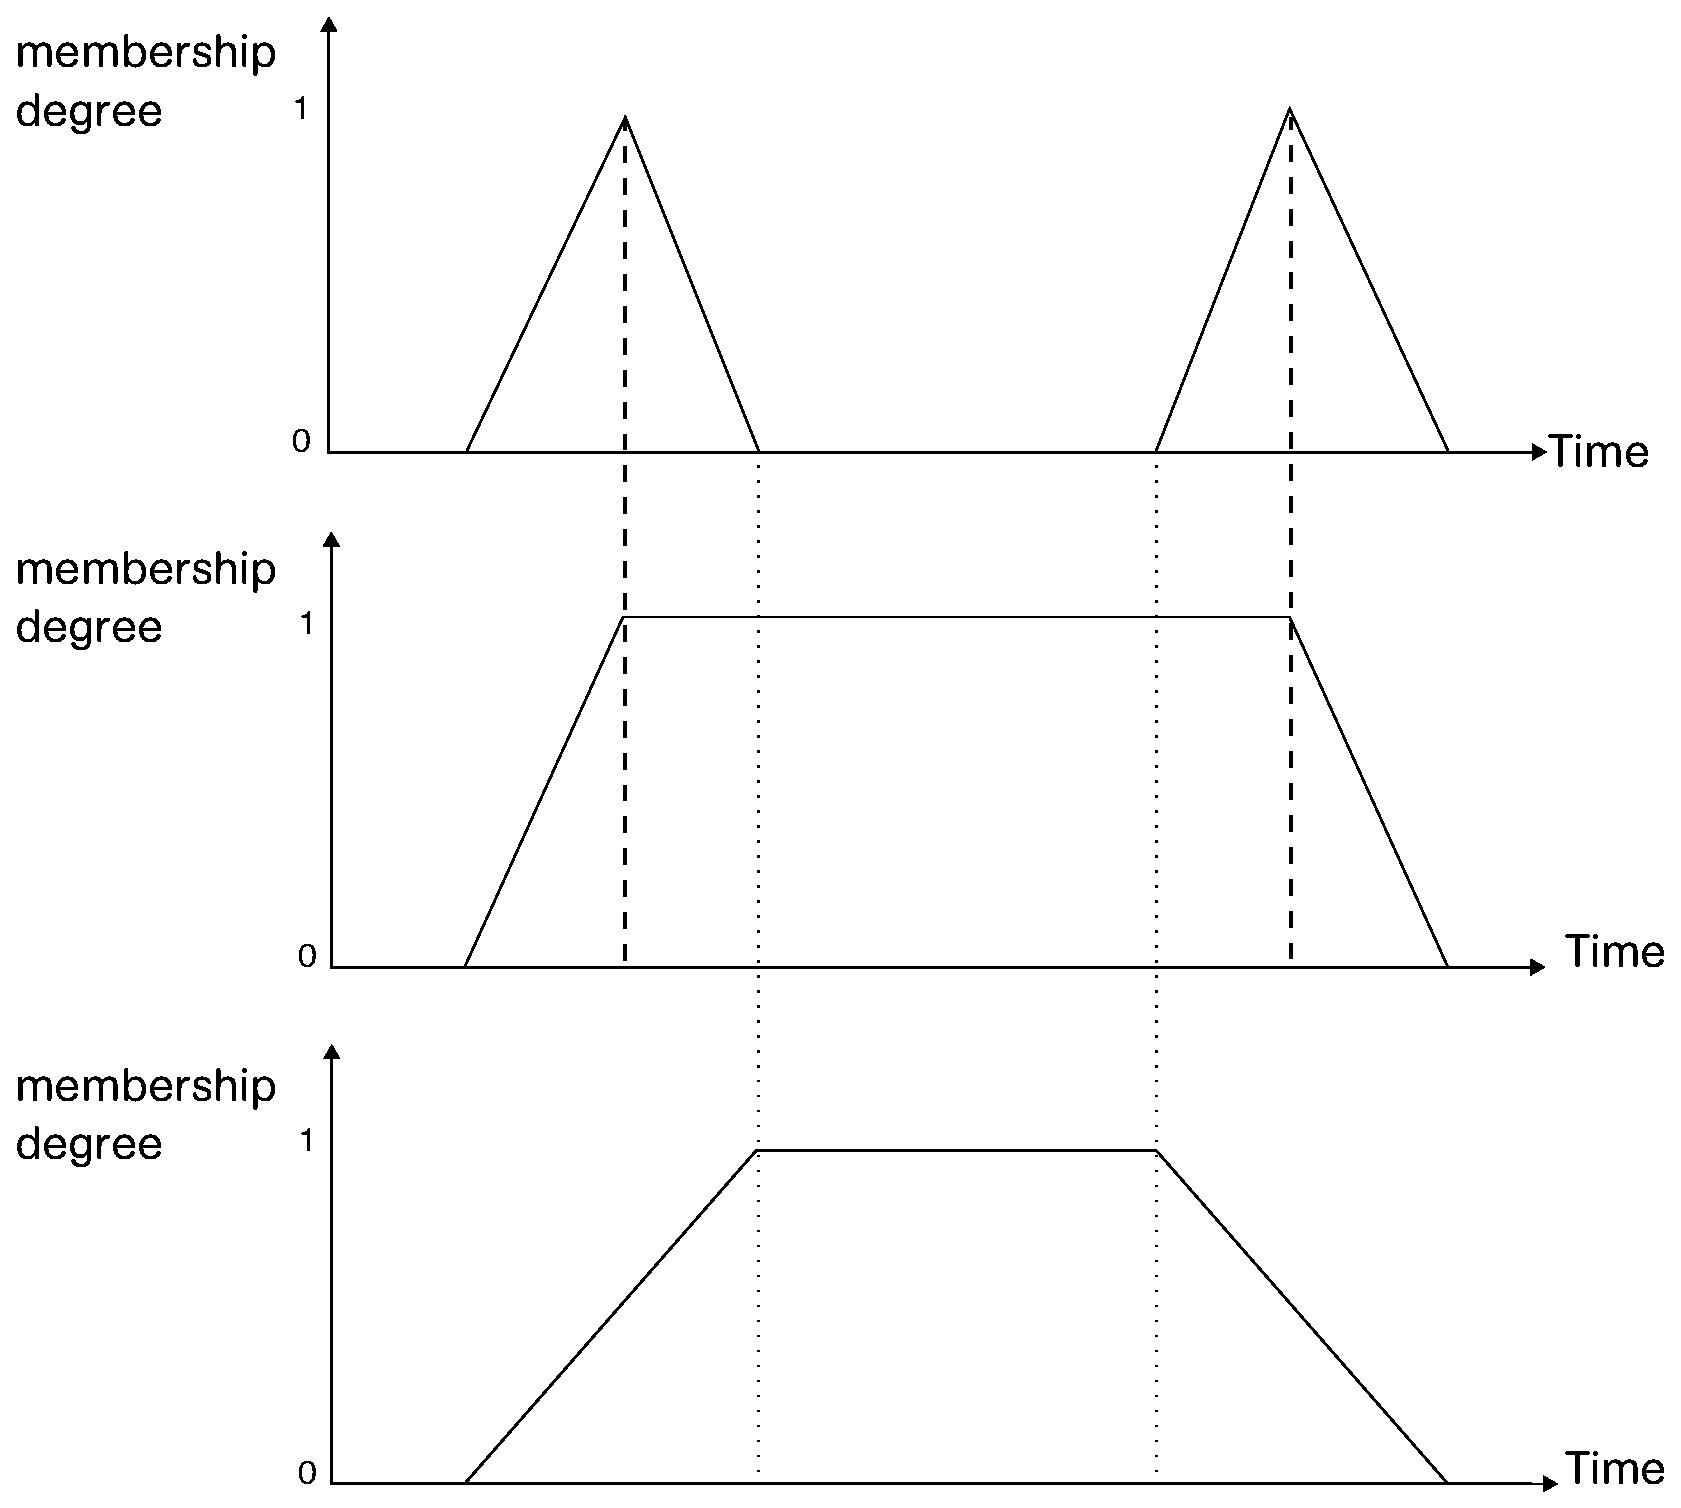
\includegraphics[scale=0.3]{graphs/trapezoidalDistribution.eps}
  \caption{Transformation to obtain the FVP. The top graph shows the two triangular possibility distributions. The middle graph shows the convex hull validity period, the bottom one shows the result of the second transformation, which maintains the imprecision.}
  \label{fig:fuzzy-validity-period}
\end{figure}
%%%%%%%%%%%%%%%%%%%%%%%%%%%%%%
% FVP
%%%%%%%%%%%%%%%%%%%%%%%%%%%%%%%



%
\section{\label{sec:proposal}Algebra for crisp temporal databases}
%
We will define the main concepts and elements in order to implement a model for temporal relational databases. First of all, we will introduce some definitions and notations.



\begin{definition}
\label{def:valid-time-relation}
\emph{Valid-time relation.}
Consider the following definitions and notations:

\begin{itemize}
 \item A set of non-temporal attributes.
	\begin{equation}
	\label{eq:attribute-set}
	A = \left \lbrace A_1, A_2, \ldots, A_n \right \rbrace
	\end{equation}
      The domain for each attribute $A_1, \ldots, A_n$ is $D_1, \ldots, D_n$ respectively. 
\item The original primary key $A_K$ is a subset of the attributes in $A$.
      \begin{equation}
       \label{eq:primary-key-a}
      A_K \subseteq A
      \end{equation}
\item Two attributes, $S$  and $E$ for the starting and ending points respectively. $I$ defines the valid time interval for the data. 
\begin{equation}
 \label{eq:attribute-time-interval}
I = \left \lbrace S, E \right \rbrace
\end{equation}

$\T$ is the time domain.

\item Then $R$, the schema for the valid-time relation is:
\begin{equation}
 \label{eq:valid-time-relation}
R = A \cup  I
\end{equation}
\item The primary key for the valid-time relation $R$ is:
\begin{equation}
 \label{eq:valid-time-temporal-pk}
PK = A_K \cup I
\end{equation}


\item We will note by $r$ any valid instance of $R$. 
      \begin{equation}
       \label{eq:valid-time-instance}
      r \subseteq D_1\ x\ \ldots\ x\ D_n x\ T x\ T
      \end{equation}


     % \end{itemize}
\item $V(t)$ is the set of all the versions for a given tuple $t$. Formally,

\begin{equation}
 \label{eq:all-the-versions}
V(t) =\left \lbrace t_i \in r, t_i\left[A_K\right] = t\left[A_K\right] \right \rbrace
\end{equation}
Obviously, $t$ itself is included in the set.
% If a tuple $t$ contains more than one version, the result of $Vt$ is a set. We will use the index $k$ to address the elements of the set. E.g. $Vt = \left \lbrace t_1, t_2, \ldots, t_n \right \rbrace$. Then $t_k , k \in \left \lbrace 1, \ldots, n \right \rbrace$ is an element of $Vt$.
\end{itemize}
\end{definition}
We will illustrate the definitions with an example.

\begin{example}
Consider the set of attributes $A = \left \lbrace A_1, A_2, A_3 \right \rbrace$. The primary key for these attributes is given by $A_K = \left \lbrace A_1, A_2 \right \rbrace$. Let $I = \left \lbrace S, E \right \rbrace$ be the set of temporal attributes that define the validity period of the data. $R$ is the valid-time relation and $r$ is an instance of the relation. The instance $r$ is given by the following elements. $r = \left \lbrace \left(a_{11}, a_{12}, a_{13}, s_1 ,e_1 \right) \right.$,  $\left(a_{21}, a_{22}, a_{23}, s_2, e_2 \right)$ , $\left. \left(a_{11}, a_{12}, a_{31}, s_3, e_3 \right) \right \rbrace$. The instance $r$ is illustrated in Table \ref{tbl:sample-definitions}. 
Consider the tuple $t_1 = \left(a_{11}, a_{12}, a_{13}, s_1 ,e_1 \right)$. Then,
\begin{align}
 \nonumber
 t_1\left[S \right]&=s_1\\
 \nonumber
t_1[E]&=e_1\\
 \nonumber
t_1[S,E]&= \left(s_1, e_1\right)\\
 \nonumber
t_1\left[A_K\right] &= \left(a_{11}, a_{12} \right) \\
 \nonumber
t_1\left[PK\right] &=\left(a_{11}, a_{12}, s_1, e_1\right)\\
 \nonumber
V(t_1) &= \left \lbrace t_1, t_3 \right \rbrace
\end{align}



\end{example}

\begin{table}[h]
\centering
%\begin{table}[htbp]
\caption[Example database for $r \in R$]{\label{tbl:sample-definitions}Example database containing the instance $r$ of the valid-time relation $R$.}
\vspace{2mm}
%\centerline{\small DATA TYPES}
\begin{tabular}{c c c c c c}\\
\hline
& \textbf{A$_1$}  & \textbf{A$_2$}  & $A_3$ & $S$ & $E$ \\
\hline
$t_1$&$a_{11}$ & $a_{12}$ & $a_{13}$ & $s_1$ & $e_1$ \\
$t_2$ & $a_{21}$ & $a_{22}$ & $a_{23}$ &  $s_2$ & $e_2$ \\
$t_3$ & $a_{11}$ & $a_{12}$ & $a_{31}$ & $s_3$ & $e_3$\\
\hline\\
\end{tabular}
\end{table}



\subsection{\label{sec:selection}Selection}
The selection operator is very useful when the user wants to obtain a subset of tuples that fulfill a certain constraint. More formally,

\begin{definition}
\label{def:crisp-selection}
 Consider the elements in definition \ref{def:valid-time-relation}.
The selection operator $\sigma$ obtains a subset of tuples that fulfill a set of constraints $P$ from an instance $r$ of the relation $R$. The set of constraints is usually a boolean combination of atomic constraints. The selection operator is noted as follows:
\end{definition}

\begin{equation}
 \label{eq:selection}
\sigma_{P} \left( r \right)
\end{equation}

Where $r \in R$ is the relation, and $P$ is the selection formula. The selection formula is a set of two elements:
% \begin{itemize}
% \item relation.attribute boolean relation relation.attribute
% \item relation.temporal-attribute allen-relation relation.temporal-attribute 
% \end{itemize}
\begin{equation}
 \label{eq:selection_formula}
P = \left \lbrace Q, Q^{T}\right \rbrace
\end{equation}

Where $Q$ is the set of non-temporal constraints and $Q^{T}$ the set of temporal constraints.
The component $Q$ is a set composed by atomic constraints: 

\begin{equation}
 \label{eq:non-temporal-constraints}
Q = \left \lbrace q_{\mbox{a}_1}  \theta \mbox{ val}_1, \ldots, q_{\mbox{a}_n}  \theta \mbox{ val}_n \right \rbrace
\end{equation}


Where:
\begin{itemize}
 \item $q_{a \in A }$ is an atomic constraint. The constraint refers to an attribute $a$ that belongs to the set of attributes $A \subseteq A_1 \ldots A_n $ of the relation $R$.
\item $\theta$ is a relational operator; usually one of $\left \lbrace =, \neq, <, \leq, >, \geq \right \rbrace$.
\item \emph{val}$_1 \ldots$\emph{val}$_n$ are values in the domain of the queried attribute. 
 \end{itemize}

The temporal constraints, $Q^t$ are provided in a similar way. The main difference is that, instead of comparisons like $\left \lbrace =, \neq, <, \leq, >, \geq \right \rbrace$, we use the Allen's relations~\cite{Allen1983}. Hence, the representation of the temporal constraints is expressed as follows:

\begin{equation}
\label{eq:temporal-constratins}
Q^{t} = \left \lbrace q_{v_1}  \AR i_1, \ldots, q_{v_n}  \AR i_n \right \rbrace
\end{equation}
Where
\begin{itemize}
\item $q_{v \in I}$ is an attribute representing a time interval. ($q_v =  \left[s_v, e_v \right]$).
\item $\AR$ is one of the thirteen Allen's relations (equal, before, overlaps, starts, finishes, meets, during) and their respective reverses (See Figure \ref{fig:allen} ).
\item $i_{x \in \left \lbrace 1 \ldots n\right \rbrace}$ is a crisp time interval with starting and ending points ($i_x = \left[s_x, e_x \right]$).

\end{itemize}


\subsubsection{\label{crisp-query-eval}Query Evaluation}
In a crisp relational database, the modelling of the query satisfaction is a boolean result. The evaluation of the query requirements results in one of two possibilities; accept the record if it satisfies all the constraints or reject the record otherwise. The evaluation of the selection formula $P$ given in equation \eqref{eq:selection_formula} is handled as follows. For each record $r$ in the database, two things happen independently:

\begin{itemize}
 \item The crisp constraints expressed in $Q$ are evaluated and aggregated. The result of this is a boolean value. We will note as $e_Q(r)$ value for the evaluation of the constraints in  $Q$ for the record $r$.
\item The temporal constraints expressed in $Q$ are evaluated and aggregated. The result of this is again a boolean value. We will note as $e_Q^{T}(r)$ the value for the evaluation of the constraints in $Q^T$ for the record $r$.
\end{itemize}

The results from $e_Q(r)$ and $e_Q^{T}(r)$ are aggregated using a boolean combination. For valid-time intervals, the preferred combination is the \emph{'and'} ($\wedge$) operator . The function $e_{\mbox{final}}\left(r\right)$ is given by:

\begin{equation}
 \label{eq:e-final-crisp}
e_{\mbox{final}}\left(r\right) = e_Q(r) \wedge e_Q^{T}(r)
\end{equation}




% Quizás mejor dejar la agregación para el caso difuso
% In order to present the results to the user, it is necessary to provide methods for both aggregation and ranking. This is explained in the following subsection.
% 
% 
% \subsubsection{\label{crisp-ranking}Aggregation and Ranking}
% In the crisp case we need to provide a method to combine the output from $Q$ and $Q^T$. That method selects or rejects a tuple 




\begin{example}
Consider an employee's database. The data are stored in two tables; Table \ref{table:employees} ($r \in R$) contains temporal data about the employees and Table \ref{table:address} ($s \in S$) contains temporal  data about the addresses for each employee. Consider now that the user wants to obtain all the employees who are a professor and that worked in the time interval $\left[7, 10 \right]$.
%\vspace{-10pt} \ref{table:employees} \ref{table:address}

\begin{table}
\centering
\caption{Employee's table. Instance $r$ of relation $R$.}
\vspace{2mm}

\begin{tabular}{c c c c c c }
\hline
ID & Job & Works for & Start & Finish \\ \hline
1 & Professor & 4 & 5 & 10 \\
2 & Technician & 4 & 3 & 7 \\
3 & Accountant & 4  & 4 & 10 \\
4 & Administrator & - & 1 & UC \\
1 & Professor & 4 & 11 & UC \\
\hline 
\end{tabular}
\label{table:employees}

%\vspace{10pt}


\end{table}

%\vspace{-25pt}

%\vspace{-10pt}

\begin{table}
\centering
r\caption{Address table. Instance $s$ of relation $S$.}
\vspace{2mm}
\begin{tabular}{c c c c }
\hline
ID & Adr. & Start & Finish \\ \hline
1 & C/ Camino de ronda & FB & 12 \\
2 & C/ Recogidas & FB & UC \\ 
3 & C/ Pintor Maldonado & FB & UC \\
4 & C/ Mesones & FB & UC \\
1 & C/ Manuel de Falla & 12 & UC \\
\hline 
\end{tabular}
\label{table:address}

%\vspace{10pt}


\end{table}

%\vspace{-25pt}

The selection formula is the following:

\begin{equation}
 \label{eq:selection-example}
\sigma_{r.Job = 'Professor', r.\left[S, E \right] \mbox{ Contains } \left[7, 10\right]} \left(r \right)
\end{equation}
The values for $e_Q(r)$ and $e_Q^T(r)$ for each record, as well as the final aggregation (see Equation \eqref{eq:e-final-crisp}) are illustrated in Table \ref{table:crisp-intermediate-calculations-employees}.
The resultset for the selection is shown in Table \ref{table:example-selection}.
\end{example}

\begin{table}
\centering
\caption[Intermediate calculations.]{Intermediate calculations for selection formula given in equation \eqref{eq:selection-example}}
\vspace{2mm}

\begin{tabular}{c c c c c c c c }
\hline
ID & Job & Works for & Start & Finish & $e_Q(r)$& $e_Q(r)$ & $e_{final}(r)$\\ \hline
1 & Professor & 4 & 5 & 10 & True & True & True\\
2 & Technician & 4 & 3 & 7 & False & False & False\\
3 & Accountant & 4  & 4 & 10 & False & True & False\\
4 & Administrator & - & 1 & UC & False & True & False\\
1 & Professor & 4 & 11 & UC & True & False & False\\
\hline 
\end{tabular}
\label{table:crisp-intermediate-calculations-employees}

%\vspace{10pt}


\end{table}


%\vspace{-10pt}

\begin{table}
\centering
\caption{Resultset table for the selection in equation \eqref{eq:selection-example}}
\vspace{2mm}
\begin{tabular}{c c c c c c }
\hline
ID & Job & Works for & Start & Finish \\ \hline
1 & Prof. & 4 & 5 & 10 \\
\hline 
\end{tabular}
\label{table:example-selection}

%\vspace{10pt}


\end{table}

%\todo[caption={crisp cartesian product}]{Maybe the cartesian product should be inside the selection??}
\subsection{\label{sec:cartesian-product}Cartesian Product}
The relational cartesian product is defined as all the possible combinations between tuples of  $r, s$ from two given relations $R$ and $S$ respectively. It is usually noted as $r \times s$.
The temporal cartesian product operator is defined as the relational cartesian product with a predicate on the temporal valid-time intervals \cite{DengfengGao2002}. The temporal cartesian product is defined then as $r \times^T s$.

We will re-define the predicate given in \cite{DengfengGao2002} in terms of the Allen's relations. To do this, two auxiliary functions should be defined.

%\todo[caption={Crisp temporal operators}]{Instead of define inline the crisp operators for intervals, Could it be more interesting to have an appendix with the implementation?}

\begin{definition}
 \label{def:crisp-intersect}
Intersect$\left(i_1, i_2 \right)$. Given two intervals $i_1$ and $i_2$, the Intersect function returns a boolean value showing whether the two intervals intersect or not. In terms of the Allen's relations, two intervals $i_1$ and $i_2$ intersect if between them exist any of the Allen's relations except Before or After. In other words, only if the Allen's relations Before or After do not hold for the two intervals, they will intersect.

\begin{equation}
 \label{eq:crisp-intersect}
\mbox{Intersect}\left( i_1, i_2 \right) = \left \lbrace \neg \left(e_1 < s_2 \right) \vee \neg \left(e_2 < s_1 \right) \right \rbrace
\end{equation}


\end{definition}


\begin{example}
Consider the following intervals $i_1 = \left[5, 10 \right]$ and  $i_2 = \left[0, 12 \right]$. The intersect operation is calculated as follows:
\begin{align}
\mbox{Intersect}\left( i_1, i_2 \right) &=& \left \lbrace \neg \left(10 < 0 \right)  \vee \neg \left(12 < 5 \right) \right \rbrace \\
\nonumber
&=& \mbox{True} \vee \mbox{True} \\
\nonumber &=& \mbox{True}
\end{align}

\end{example}

The other auxiliary function that allows to define the predicate for the cartesian product, needs some previous definitions as well. 

\begin{definition}
 \label{def:crisp-last}
Last$\left(i_p, i_q \right)$. Given two time points $i_p$ and $i_q$, this function obtains the greatest time point.
\begin{equation}
 \label{eq:last-crisp}
\mbox{Last}\left(i_p, i_q \right) = 
\begin{cases}
i_p & \mbox{ if } i_p \mbox{ after } i_q \\
i_q & \mbox{ otherwise } 
\end{cases}
\end{equation}
Note that because both $i_p, i_q$ are time points, the after relation is implemented as $i_p > i_q$.
\end{definition}

\begin{definition}
 \label{def:crisp-first}
First$\left(i_p, i_q \right)$. Given two time points $i_p$ and $i_q$, this function obtains the least time point.
\begin{equation}
 \label{eq:first-crisp}
\mbox{First}\left(i_p, i_q \right) =
\begin{cases}
i_p & \mbox{ if } i_p \mbox{ before } i_q \\
i_q & \mbox{ otherwise } 
\end{cases}
\end{equation}
Note that because both $i_p, i_q$ are time points, the before relation is implemented as  $i_p < i_q$.
\end{definition}



\begin{definition}
 \label{def:crisp-overlapping-interval}
Overlapping-interval$\left(i_1, i_2 \right)$. Given two intervals $i_1 = \left[s_1, e_1 \right]$ and $i_2 = \left[s_2, e_2\right]$, this function returns an overlapping interval from the original two intervals.
\begin{equation}
 \label{eq:crisp-overlapping-interval}
\mbox{OvInt}\left(i_1, i_2 \right) = 
\begin{cases}
\left[\mbox{Last}\left( s_1, s_2 \right), \mbox{First}\left(e_1, e_2 \right) \right] & \mbox{ if } \mbox{Last}\left( s_1, s_2 \right) \leq \mbox{First}\left(e_1, e_2 \right) \\
\emptyset & \mbox{ otherwise } 
\end{cases}
\end{equation}
\end{definition}

Now it is possible to define the temporal cartesian product.

\begin{definition}
 \label{def:crisp-temporal-cartesian-product}
Temporal Cartesian Product. Consider the elements in definition \ref{def:valid-time-relation}.
The temporal cartesian product of two temporal relations $r \in R = \left(A_1, \ldots A_n, S, E \right)$ and $s \in S = \left(B_1 \ldots, B_m, S, E \right)$ is noted as $r \times^T s$ and is defined by the following formula:

\begin{align}
 \label{eq:crisp-temporal-cartesian-product}
r \times^T s =  \lbrace z^{\left(n+m+2 \right)} | \exists x \in r, \exists y \in s \\
\nonumber
\mbox{intersect}\left(x[S,E], y[S,E] \right) \wedge \\
\nonumber
z\left[A\right] = x\left[A\right] \wedge z\left[B\right] = y \left[B \right] \wedge \\
\nonumber
 z\left[S, E \right] = \mbox{OvInt}\left(x\left[S, E\right], y\left[S, E\right] \right) \wedge z\left[S, E\right] \neq \emptyset  \rbrace
\end{align}
Where $A$ and $B$ are a shorthand for $\left \lbrace A_1, \ldots A_n\right \rbrace$ and $\left \lbrace B_1 \ldots, B_m\right \rbrace$ respectively.
\end{definition}

The following example illustrates the temporal cartesian product.
\begin{example}
 \label{ex:crisp-temporal-cartesian-product}
Consider the employee's database mentioned before (Tables \ref{table:employees} and \ref{table:address}). Table \ref{table:example-crisp-cartesian-product} illustrates an intermediate step to compute the temporal cartesian  product.



\end{example}

\begin{table}
\begin{center}
\caption{Intermediate calculations for the temporal cartesian product.}
\vspace{2mm}
\begin{tabular}{c c c c c c c c}
\hline
r.id & s.id & $x\left[S, E\right]$ & $y\left[S, E\right]$ & $^1$ & $^2$ & $^3$  &$z\left[S, E \right]$  \\ \hline
1 & 1 & $\left[5, 10 \right]$  & $\left[FB, 11 \right]$  & True  & 11 &  5 & $\left[5, 11 \right]$ \\
1 & 2 & $\left[5, 10 \right]$  & $\left[FB, UC \right]$  & True  & UC &  5 & $\left[5, UC \right]$ \\
1 & 3 & $\left[5, 10 \right]$  & $\left[FB, UC \right]$  & True  & UC &  5 & $\left[5, UC \right]$ \\
1 & 4 & $\left[5, 10 \right]$  & $\left[FB, UC \right]$  & True  & UC &  5 & $\left[5, UC \right]$ \\
1 & 1 & $\left[5, 10 \right]$  & $\left[12, UC \right]$  & False & UC & 12 & -                     \\
2 & 1 & $\left[3, 7 \right]$   & $\left[FB, 11 \right]$  & True  & 11 &  3 & $\left[3, 11 \right]$ \\
2 & 2 & $\left[3, 7 \right]$   & $\left[FB, UC \right]$  & True  & UC &  3 & $\left[3, UC \right]$ \\
2 & 3 & $\left[3, 7 \right]$   & $\left[FB, UC \right]$  & True  & UC &  3 & $\left[3, UC \right]$ \\
2 & 4 & $\left[3, 7 \right]$   & $\left[FB, UC \right]$  & True  & UC &  3 & $\left[3, UC \right]$ \\
2 & 1 & $\left[3, 7 \right]$   & $\left[12, UC \right]$  & False & UC & 12 &  -                    \\
3 & 1 & $\left[4, 10 \right]$  & $\left[FB, 11 \right]$  & True  & 11 &  4 & $\left[4, 11 \right]$ \\
3 & 2 & $\left[4, 10 \right]$  & $\left[FB, UC \right]$  & True  & UC &  4 & $\left[4, 11 \right]$ \\
3 & 3 &  $\left[4, 10 \right]$ & $\left[FB, UC \right]$  & True  & UC &  4 & $\left[4, 11 \right]$ \\
3 & 4 & $\left[4, 10 \right]$  & $\left[FB, UC \right]$  & True  & UC &  4 & $\left[4, 11 \right]$ \\
3 & 1 & $\left[4, 10 \right]$  & $\left[12, UC \right]$  & False & 12 & 12 & -                     \\
4 & 1 & $\left[1, UC \right]$   & $\left[FB, 11 \right]$ & True  & UC &  1 & $\left[1, UC \right]$ \\
4 & 2 & $\left[1, UC \right]$   & $\left[FB, UC \right]$ & True  & UC &  1 & $\left[1, UC \right]$ \\
4 & 3 & $\left[1, UC \right]$   & $\left[FB, UC \right]$ & True  & UC &  1 & $\left[1, UC \right]$ \\
4 & 4 & $\left[1, UC \right]$   & $\left[FB, UC \right]$ & True  & UC &  1 & $\left[1, UC \right]$ \\
4 & 1 & $\left[1, UC \right]$   & $\left[12, UC \right]$ & True  & UC & 12 & $\left[12, UC \right]$ \\
1 & 1 & $\left[11, UC \right]$  & $\left[FB, 11 \right]$ & False & UC & 11 & -                      \\
1 & 2 & $\left[11, UC \right]$  & $\left[FB, UC \right]$ & True  & UC & 11 &  $\left[11, UC \right]$ \\
1 & 3 & $\left[11, UC \right]$  & $\left[FB, UC \right]$ & True  & UC & 11 & $\left[11, UC \right]$ \\
1 & 4 & $\left[11, UC \right]$  & $\left[FB, UC \right]$ & True  & UC & 11 & $\left[11, UC \right]$ \\
1 & 1 & $\left[11, UC \right]$  & $\left[12, UC \right]$ & True  & UC & 12 &  $\left[12, UC \right]$ \\
\hline 
\end{tabular}
\label{table:example-crisp-cartesian-product}
\end{center}
$^1$, intersect$\left(x\left[S, E\right], y\left[S, E\right]\right)$\\
$^2$, First$\left(x[E], y[E] \right)$ \\
$^3$, Last$\left(x[S], y[S] \right)$
\end{table}

\subsubsection{\label{sec:join}Join}
The join operator $\Join$ builds a new relation from two given relations, namely $r \in R$ and $s \in S$. This new relation is a set with all the possible combinations of tuples in both $r$ and $s$ that fulfill a predicate. It is usually noted as $r \Join_{a \theta b} s$ and called (theta) join, where $a,b$ are attributes from $r$ and $s$ respectively and $\theta$ a relational operator. The temporal join definition is based on the temporal cartesian product.

\begin{definition}
 \label{def:temporal-theta-join}
Temporal theta join. Let $r$ and $s$ be two  instances of relations $R, S$ respectively. Then the temporal theta join is defined as follows:
\begin{equation}
 \label{eq:temporal-theta-join}
r \Join_{a \theta b}^{T} s= \sigma_{a \theta b} \left(r \times^T s \right)
\end{equation}

\end{definition}


% _{\begin{figure}
%  \includegraphics[scale=0.60]{graphs/innerjoin.eps}
% \caption[Comparison inner join vs temporal inner join.]{\label{fi:innerjoin} Comparison between the relational (non-temporal) inner join (left graph) and the temporal inner join (right graph).}
% \end{figure}
% 
% 
% 
% Figure \ref{fi:innerjoin} compares the relational inner join with respect to the temporal inner join. The right graph illustrates the temporal case. It is clear that the temporal inner join is a subset or is equal to the relational inner join.}

% \subsubsection{\label{subsec:Equijoin}Equijoin}
% The equijoin operator for relational databases enforces equality between specified subsets of the attributes of the relations. Then, the temporal equijoin operator is defined as the temporal join operator.
% 
% \begin{definition}
%  \label{def:equijoin}
% Equijoin. Let $R$ and $S$ be two relations and $r, s$ be the instances of each relation respectively. $A , B$ are the sets of the attributes for the relations $R$ and $S$ respectively. And let $A' \subseteq A$ and $B' \subseteq B$. Then, the temporal equijoin is defined as follows:
% \begin{equation}
%  \label{eq:equijoin}
% r \Join_{r\left[A' \right] = s\left[B' \right]}^{T} s =  \sigma_{r\left[A' \right] = s\left[B' \right]} \left(r \times^T s \right)
% \end{equation}
% \end{definition}
% 
% 
% \subsubsection{\label{subsubsec:temporal-equijoin}Temporal Equijoin}
% The temporal equijoin is an equijoin operator in which the subset of attributes in the equijoin condition, are part of the primary key. Hence, the operator is defined as follows:
% 
% \begin{definition}
% \label{def:temporal-equijoin}
% Temporal equijoin ($r \mbox{ TE-join } s$). Let $R, S$ be two relations and $r, s$ the instances of each relation respectively. Consider that $PK$ is the primary key of both relations. The temporal equijoin operator is defined as follows:
% \begin{equation}
%  \label{eq:temporal-equijoin} 
% r \mbox{ TE-join } s \equiv r \Join_{r\left[PK\right] = s\left[PK\right]}^{T} s
% \end{equation}
% \end{definition}
% 
% \subsubsection{\label{subsec:natural-join}Natural Join}
% The temporal natural join is a temporal equijoin on identically named attributes.
% 
% \begin{definition}
%  \label{def:temporal-natural-join}
% Temporal natural join. Consider the following relations $R = \left(A_1, \ldots, A_n, C_1, \ldots, C_k, S, E \right)$ and $S = \left(B_1, \ldots, B_m, C_1, \ldots, C_k, S, E \right)$. Let $r,s$ be instances of $R, S$ respectively. The temporal natural join is defined as follows:
% \begin{equation}
%  \label{eq:temporal-natural-join}
% r \Join^T s = r \Join_{r\left[C_1\right] = s\left[C_1\right] \wedge \ldots \wedge r\left[C_k\right] = s\left[C_k\right]} s
% \end{equation}
% \end{definition}

% \todo[caption={outer-joins}]{Still have to define the outer joins implementation...}
% \subsubsection{\label{subsec:outer-joins}Outer Joins}
% 
% 
% \begin{figure}
%  \includegraphics[scale=0.60]{graphs/outerjoin.eps}
% \caption{\label{fi:outerjoin} Comparison between a left outer join (left graph) and a right inner join (right graph).}
% \end{figure}


\subsection{Projection}
\subsection{Cartesian Product}
\subsection{Union}
\subsection{Difference}
\subsection{Intersection}
\subsection{Join}
\subsection{Division}

\section{Algebra for (fuzzy) temporal databases}
\begin{definition}
\label{def:generalized-fuzzy-temporal-domain}
\emph{Generalized fuzzy temporal domain.}
Consider $\T$ to be the temporal domain, and let $\tilde \Pow\left( \T\right)$ be the set of all \emph{normalized} possibility distributions (see Section \ref{subsec:possibility-theory}, equation \eqref{NormalizationProperty}) defined on $\T$.
The Generalized Fuzzy Temporal Domain, $\T_G$ is
\begin{equation}
\T_G \subseteq \left \lbrace \tilde \Pow\left( \T\right) \cup \text{NULL} \right \rbrace
\end{equation}
\end{definition}

Note that $\T_G \subseteq D_G$. The datatypes for this domain have been studied previously in section \ref{sec:time-rep} and are shown in tables \ref{tbl:time-point-types} and \ref{tbl:time-interval-types}.

A generalized fuzzy relation is defined in \cite{Medina1994}. Here, we will extend the definition to a generalized fuzzy temporal relation.

\begin{definition}
\emph{Generalized fuzzy temporal relation.}
\label{def:fuzzy-temporal-relation}
Consider the elements in definition \ref{def:valid-time-relation}. Some of them will be extended for the fuzzy case.

\begin{itemize}
%  \item A set of non-temporal fuzzy  or crisp attributes.
% 	\begin{equation}
% 	\label{eq:fuzzy-attribute-set}
% 	A = \left \lbrace A_1, A_2, \ldots, A_n \right \rbrace
% 	\end{equation}
%       The domain for each attribute $A_1, \ldots, A_n$ is $D_1, \ldots, D_n$ respectively. 
% \item The primary key $A_K$ is a subset of $A$.
%       \begin{equation}
%        \label{eq:fuzzy-primary-key-a}
%       A_K \subset A
%       \end{equation}
% A formal definition of primary key for fuzzy relational databases will be given later in Definition \ref{def:generalized-primary-key}.
% \item A set of two attributes; $S$  and $E$ the attributes for the starting and ending ill-known points respectively. $I$ is a possibilistic validity period \emph{PVP} as explained in Section \ref{subsec:ill-known-interval}.
% \begin{equation}
%  \label{eq:fuzzy-attribute-time-interval}
% I = \left \lbrace S, E \right \rbrace
% \end{equation}
\item An attribute called version identifier, $V_{ID}$, will be added to the schema. This attribute is a counter for each different version of the entities. 
% \begin{equation}
%  \label{eq:fuzzy-version-identifier}
% V_{ID} \subset \N
% \end{equation}



\item Then $R_{FTG}$, the schema for the fuzzy valid-time relation is:
\begin{equation}
 \label{eq:fuzzy-valid-time-relation}
R_{FTG} = A \cup V_{ID} \cup  I
\end{equation}
\item The primary key for the fuzzy valid-time relation $R_{FTG}$ is:
\begin{equation}
 \label{eq:fuzzy-valid-time-temporal-pk}
K_{GT} = A_K \cup V_{ID}
\end{equation}
A formal definition of the primary key for fuzzy valid-time relations will be given later in Definition \ref{def:generalized-fuzzy-temporal-key}.


\item We will note by $r$ any valid instance of $R_{FTG}$. 
      \begin{equation}
       \label{eq:fuzzy-valid-time-instance}
      r \subseteq D_1\ x\ \ldots\ x\ D_n
      \end{equation}

% \item Let $t$ be a tuple in the instance $r$; $t \in r$:
%       \begin{itemize}
%       \item We will note the values for the starting and the ending  points,$s$ and $e$  respectively. The value for the time interval is given by $i$.
%       \begin{align}
%        \label{eq:fuzzy-starting-point}
%       s = t\left[S \right]\\
%       e = t\left[E \right]\\
%       i = \left(s, e\right)
%       \end{align}
% 
% 
%       \item Let $A_k \subset A$ be the set of the non-temporal attributes that are part of the primary key (equation \eqref{eq:fuzzy-primary-key-a}). Then, $a_k$ denotes the values for the non-temporal attributes of the primary key.
% 	    \begin{equation}
% 	     \label{eq:fuzzy-pk-attribute} 
% 	      a_k = t\left[A_K \right]
% 	    \end{equation}
% 
    \item Let $K_{GT}$ be the primary key for the valid-time relation as given in equation \eqref{eq:fuzzy-valid-time-temporal-pk}. Then, $k$ denotes the values for the attributes in the primary key.
	  \begin{equation}
	   \label{eq:fuzzy-value-pk}
	  k = t\left[K_{GT} \right]
	  \end{equation}
% 
% 
%       \end{itemize}
% \item $Vt$ is the set with all the versions for a given tuple $t$.
% 
% \begin{equation}
%  \label{eq:fuzzy-all-the-versions}
% Vt = r\left(t\left[A_K\right] \right)
% \end{equation}
% If a tuple $t$ contains more than one version, the result of $Vt$ is a set. We will use the index $k$ to address the elements of the set. E.g. $Vt = \left \lbrace t_1, t_2, \ldots, t_n \right \rbrace$. Then $t_k , k \in \left \lbrace 1, \ldots, n \right \rbrace$ is an element of $Vt$.
\end{itemize}
%\end{definition}

We will illustrate the definitions with an example.

\begin{example}
Consider the set of attributes $A = \left \lbrace A_1, A_2, A_3 \right \rbrace$. The primary key for these attributes is given by $A_K = \left \lbrace A_1, A_2 \right \rbrace$. Let $I = \left \lbrace S, E \right \rbrace$ be the set of temporal attributes that define the possibilistic validity period of the data. $R_{FTG} = A \cup V_{ID} \cup I$ is the valid-time relation and $r$ is an instance of the relation. The instance $r$ is given by the following elements. $r = \left \lbrace \left(a_{11}, a_{12}, a_{13}, 001, s_1 ,e_1 \right) \right.$,  $\left(a_{21}, a_{22}, a_{23}, 001, s_2, e_2 \right)$ , $\left. \left(a_{11}, a_{12}, a_{31}, 002, s_3, e_3 \right) \right \rbrace$. The instance $r$ is illustrated in Table \ref{tbl:fuzzy-sample-definitions}. 
Consider the tuple $t = \left(a_{11}, a_{12}, a_{13}, s_1 ,e_1 \right)$. Then,
\begin{align}
 \nonumber
s_1 &= t\left[S \right]\\
 \nonumber
e_1 &= t[E]\\
 \nonumber
i\ \ &= \left(s_1, e_1\right)\\
 \nonumber
a_k &= t\left[A_K\right] = \left(a_{11}, a_{12} \right) \\
 \nonumber
k &= t\left[PK\right] =\left(a_{11}, a_{12}, s_1, e_1\right)\\
 \nonumber
Vt &= r\left(t\left[A_K\right] \right) = \left \lbrace t_1, t_3 \right \rbrace
\end{align}



\end{example}

\begin{table}[h]
\caption[Example of fuzzy valid-time relation.]{\label{tbl:fuzzy-sample-definitions}Sample database containing the instance $r$ of the fuzzy valid-time relation $R_{FTG}$.}
\centering
\begin{tabular}{c c c c c c c}\\ \hline
& \textbf{A$_1$}  & \textbf{A$_2$}  & $A_3$ & $V_{ID}$ & $S$ & $E$ \\
\hline
$t_1$&$a_{11}$ & $a_{12}$ & $a_{13}$ & $001$ & $s_1$ & $e_1$ \\
$t_2$ & $a_{21}$ & $a_{22}$ & $a_{23}$& $001$ &  $s_2$ & $e_2$ \\
$t_3$ & $a_{11}$ & $a_{12}$ & $a_{31}$& $002$ & $s_3$ & $e_3$\\
\hline\\
\end{tabular}
\end{table}



% 
% 
% Consider $\A$ to be the set of all the entities, and let $A=\left(A_1, \ldots, A_n \right), A \in \A$ be the set of (fuzzy) attributes that define an entity. Let $\I_{PVP}$ be the set of all the ill-known time intervals and let $I = \left(X, Y \right)$ be a PVP, $I \in \I_{PVP}$.  The pair $\left(A, I\right)$ expresses that the data regarding the entity A are valid during the ill-known time interval I. Let $R_{FTG} \subseteq \A \  x\  \I_{PVP}$ be a valid-time relation. Then, the following equation indicates that the pair $\left(A, I\right)$ is in the relation R:
% 
% \begin{equation}
% \label{eq:fuzzy-rel-def}
% \left( R_{FTG}, \left(A , I\right) \right)
% \end{equation}
% 
 A generalized fuzzy temporal relation $R_{FTG}$ can be noted also by:
\label{def:generalized-fuzzy-temporal-relation}
\begin{equation}
\label{eq:generalized-fuzzy-temporal-relation}
R_{FTG} = \left(\Head, \Body \right)
\end{equation}
Where $\Head$ is the Head of the relation and consist on a fixed set of triplets attribute- domain - compatibility with an optional the valid-time attribute:

\begin{align}
\label{eq:head-valid-time}
\Head = \big \lbrace \left(A_{G1}:D_{G1}\left[,C_{A_{G1}} \right] \right),\\
\nonumber
 \ldots,\\
 \nonumber
  \left(A_{Gn}:D_{Gn}\left[,C_{A_{Gn}} \right] \right),\\
  \nonumber
  \Big[  \left( \text{PVP}, D_{\text{PVP}}\left[,C_{A_{\text{PVP}}} \right] \right) \Big] \big \rbrace
\end{align}
Note that $D_{Gj}$ ($j = 1, \ldots, n$) is the domain for the attribute $A_{Gj}$. $C_{A_{Gj}}$ is the compatibility attribute in the unit interval $\left[0, 1 \right]$.

$\Body$ is the body of the relation and it consists on a set of tuples. Each tuple is a triplet attribute- value- degree with an optional valid-time attribute:

\begin{align}
\label{eq:body-valid-time}
\Body = \big \lbrace \left(A_{G1}:\tilde{d}_{i1}\left[,c_{i1} \right] \right),\\
\nonumber
 \ldots,\\
 \nonumber
  \left(A_{Gn}:\tilde{d}_{in}\left[,c_{in} \right] \right),\\
  \nonumber
   \Big[  \left( \text{PVP}, \tilde{d}_{\text{PVP}} \left[,C_{A_{\text{PVP}}} \right] \right)  \Big] \big \rbrace
\end{align}

\end{definition}


The definition in \cite{Medina1994} for $R_{FTG}$ shows that classical relations are a particular case of this model. 

\subsection{\label{subsection:fuzzy-selection}Selection}
The selection operator is defined analogously as the crisp selection operator given in Definition \ref{def:crisp-selection} and the formal specification given by equation \eqref{eq:selection}. 
%In order to distinguish the possibilistic selection from the crisp selection, the possibilistic operators will be written with the superscript FT.


\begin{definition}
\label{def:poss-selection}
 Consider the elements in definition \ref{def:fuzzy-temporal-relation}.
The selection operator $\tilde\sigma^{T}$ returns a subset of tuples that fulfill a set of constraints $P$ from an instance $r$ of the relation $R$. The set of constraints is usually a boolean combination of atomic constraints. The selection operator is noted as follows:
\end{definition}

\begin{equation}
 \label{eq:poss-selection}
\tilde\sigma^{\mbox{T}}_{P} \left( r \right)
\end{equation}

Where $r \in R$ is the relation, and $P$ is the selection formula. 


In the possibilistic model, the main modification is that the selection predicate $P$ is not a boolean function. The selection predicate $P$ returns a satisfaction degree (in the unit interval). 
The selection formula has the same appearance than the crisp selection formula in equation \eqref{eq:selection_formula}:
\begin{equation}
 \label{eq:fuzzy-selection_formula}
P = \left \lbrace Q, Q^{T}\right \rbrace
\end{equation}

In this case, in order to evaluate both, where  $Q$ and $Q^{T}$ could be fuzzy or crisp predicates, it is necessary to define the evaluation functions for both $Q$ and $Q^{T}$. We will illustrate the possibilistic evaluation of $Q$. The possibilistic evaluation of $Q^T$ is analogous. First of all, consider a boolean function $\bool:\Boolean^{n}  \rightarrow \Boolean$. The evaluation function for the constraints in $Q$  is given by:

\begin{equation}
 \label{eq:evaluation-function}
\lambda : Q \rightarrow \Boolean : \lambda (Q) \rightarrow \bool \left(q_{a_1}  \theta \mbox{ val }, \ldots, q_{a_n}  \theta \mbox{ val } \right)
\end{equation}

Now, the uncertainty about the evaluation of $Q$ and a boolean function $\bool:\Boolean^{n}  \rightarrow \Boolean$ is given by:

\begin{equation}
 \label{eq:evaluation-lambda-function}
\pi_{\lambda \left(Q \right)} = \tilde{\bool} \left(\pi_{q_{a_1}  \theta \mbox{ val }}, \ldots, \pi_{q_{a_n}  \theta \mbox{ val }} \right)
\end{equation}




% The temporal constraints, $Q^t$ are provided in a similar way. The main difference is that, instead of comparations like $\left \lbrace =, \neq, <, \leq, >, \geq \right \rbrace$, we use the allen's relations. Hence, the representation of the temporal constraints is expressed as follows:
% 
% \begin{equation}
% \label{eq:temporal-constratins}
% Q^{t} = \left \lbrace q_{v_1}  ar \mbox{ val }, \ldots, q_{v_n}  ar \mbox{ val } \right \rbrace
% \end{equation}
% Here, $ar$ is one of the thirdteen Allen's relations (equal, before, overlaps, starts, finishes, meets, during) and their respective reverses.


\subsubsection{Query Evaluation}
In fuzzy querying of regular (relational) databases, the modelling of query satisfaction is a matter of degree. Usually, the evaluation of the query requirements for a record results in a satisfaction degree $s$, where $s$ lies in $\left[0,1\right]$, where 0 denotes total dissatisfaction and 1 denotes complete satisfaction. In crisp querying, the evaluation of query requirements for a record results in the accepting or rejecting of the record as a part of the result set. This can be modelled using satisfaction degrees, by assigning rejection a degree of $0$ and acceptance a degree of $1$ and not using any other value in $\left[0,1\right]$.

The evaluation of the predicate $P = \left( Q, Q^T \right)$, is now handled as follows. For each record $r$ in the database, with the valid-time notion of $r$ being specified by a PVP $J$, two events happen independently:


\begin{itemize}
\item
The preferences expressed in $Q$ are evaluated, resulting in a satisfaction degree denoted here $e_{Q}(r)$. The presented model accepts any sound way of calculating this evaluation, as long as $e_{Q}(r) \in \left[0,1\right]$. 
\item
Depending on the Allen Relation selected ($\AR$), a specific set of ill-known constraints is considered. The possibility and necessity that $r$ fulfills all these constraints are calculated using formulas based on equations \eqref{ill-known-pos} respectively \eqref{ill-known-nec} and aggregated using the $\min$ operator. 
\end{itemize}



\subsubsection{Aggregation and Ranking}
In order to present the results to the user, a crude ranking method is used: for every record $r$, the sum of $\Pos_{Q^{time}}(r)$ and $\Nec_{Q^{time}}(r)$ gives an evaluation score $e'_{Q^{time}}(r)$ in interval $\left[0,2\right]$. Because necessity cannot exceed $0$ unless possibility is $1$, this gives a natural ranking score. Some authors ~\cite{Bosc2010a} mentioned before that the possibility and necessity measures result in a total order in the set of events.  This $e'_{Q^{time}}(r)$ is then rescaled to the unit interval, resulting in $e_{Q^{time}}(r)$. The final ranking $e_{final}(r)$ is now given by a convex combination:


\begin{equation}
\label{eq:convex-comb}
e_{final}(r)\ =\ \omega*e_{Q}(r)\ +\ (1-\omega)*e_{Q^{time}}(r), \omega \in \left[0, 1 \right]
\end{equation}

The use of this convex combination allows a record to make up for a low score for the temporal constraint by a good score for the non-temporal constraint (or vice versa). Changing $\omega$ also allows granting the temporal constraint more weight with respect to the non-temporal constraint (or vice versa).

\begin{example} 
Consider the example relation $c \in C$ given in Table \ref{tb:car-models} describing car models, containing general attributes (model name, manufacturer, car segment) and one PVP  describing the approximate period of time during which the car model was sold. In this example, the value for $D$ is stored in \emph{yyyy} format and $a$ and $b$ are represented by an integer. The ID field identifies a car model while the field Instance ID (IID) identifies the instance for a car model, thus a car model in a certain state.
\end{example}


\begin{table}[h]
\centering
\caption{Example database, instance $c \in C$}
\vspace{2mm}
\begin{tabular}{c c c c c c c}
\hline
ID & IID & Segment & Manufacturer & Name & Start & End  \\ [0.5ex]
\hline
001 & 1 & B & Peugeot & 205 & [1985,2,3] & [1997,2,1] \\
002 & 1 & C & Peugeot & 305 & [1977,2,2] & [1989,2,3] \\
003 & 1 & B & Citroen & C2 & [2001,1,1] & [2005,1,1] \\
001 & 2 & B & Peugeot & 206 & [2000,1,2] & [2011,2,1] \\
001 & 3 & B & Peugeot & 207 & [2006,1,1] & [2011,1,1]\\
\hline
\end{tabular}
%\vspace{10pt}
\label{tb:car-models}
%\vspace{-30pt}
\end{table}

Consider the following query:
\begin{center}
\emph{The user wants to obtain a list of models from segment B, sold by manufacturer Peugeot before the Citroen C2.}\\
\end{center}

Using the introduced notations in \eqref{eq:poss-selection},\eqref{eq:fuzzy-selection_formula}, the query is translated to: 
\begin{equation}
\tilde \sigma^{\mbox{T}}_{\left \lbrace Q, Q^T\right \rbrace} \left( c \right)\
\end{equation}

The query constraints are the following:

\begin{align}
Q & = \left(c.Segment =  B\right) \wedge \left(c.Manufacturer = Peugeot\right)\\
Q^{T} & = c.\left[S, E \right] \mbox{Before} \left[2001,1,1\right], \left[2005,1 ,1 \right]
\end{align}


\begin{table}[ht]
\caption{Result table and ranking}
\centering
\begin{tabular}{c c c c c c c}
\hline
ID & IID &  $\Pos_{Q^{T}}$ & $\Nec_{Q^{T}}$ & $e_{Q^{T}} (rescaled)$ & $Q$ & $e_{final}$ ($\omega=0.5$) \\ [0.5ex]
\hline
001 & 1 & 1 &  1 & 1 & 1 & 1 \\
002 & 1 & 1 & 1 & 1 & 0.5 & 0.75 \\
003 & 1 & 1 & 0.5 & 0.75 &0 & 0.375\\
001 & 2 & 1 & 0 & 0.5 &1 & 0.75 \\
001 & 3 & 0 & 0 & 0 &1 & 0.5\\
\hline
\end{tabular}
\label{tb:results}
\end{table}

Table \ref{tb:results} shows a natural and gradual ranking for the results. The last record, (ID 001, IID 3) shows also that with $\omega$ = 0.5 both temporal and regular criteria have the same importance.

\subsection{\label{subsection:fuzzy-cartesian-product}Cartesian Product}

In this subsection we are going to extend the crisp version of the temporal cartesian product to deal with ill-known time intervals. First of all, we need to define the ill-known counterpart functions of the previously defined \emph{intersects, first, last, OvIn}.

\begin{definition}
 \label{def:ik-intersects}
Two ill-known time intervals intersect if one or both of the before and after relationships do not hold. Consider $I = \left[I_s, I_e \right]$ and $J = \left[J_s, J_e \right]$ be two ill-known time intervals with $I_s, J_s$ the starting ill-known points and $I_e, J_e$ the ending ill-known points of the intervals. Let the following ill-known constraints:
\begin{align}
 \label{eq:ik-intersects}
C_1 &=& \left(<, I_s \right)  \\
C_2 &=& \left(=, J_s \right) \\
C_3 &=& \left(<, J_s \right) \\
C_4 &=& \left(=, I_s \right) \\
\mbox{Intersects}\left(I, J\right) &=& \left \lbrace \neg \left(C_1 \wedge C_2 \right) \vee  \neg \left( C_3 \wedge C_4 \right)  \right \rbrace \\
\nonumber
&=& \left \lbrace \neg \left( \left(C_1 \wedge C_2 \right) \wedge \left(C_3 \wedge C_4 \right)  \right)\right \rbrace
\end{align}
\end{definition}


\begin{definition}
 \label{def:ik-last}
Last$\left(I_n, J_m \right)$. Given two ill-known points $I_n$ and $I_m$, the last operator is a combination of the following ill-known constraints:
\begin{align}
 \label{eq:il-last}
C_1 &=& \left(>, I_n \right) \\
C_2 &=& \left(=, J_m \right) \\
C_3 &=& \left(>, J_m \right) \\
C_4 &=& \left(=, I_n \right) \\
\mbox{Last}\left(I_n, J_m \right) &=& \left(C_1 \wedge C_2  \right) \vee \left(C_3 \wedge C_4 \right)
\end{align}
\end{definition}

Analogously, the first operator is defined as follows.
\begin{definition}
 \label{def:ik-first}
First$\left(I_n, J_m \right)$. Given two ill-known points $I_n$ and $I_m$, this operator is a combination of the following ill-known constraints:
\begin{align}
 \label{eq:ik-first}
C_1 &=& \left(<, I_n \right)\\
C_2 &=& \left(=, J_m \right)\\
C_3 &=& \left(<, J_m \right) \\
C_4 &=& \left(=, I_n \right) \\
\mbox{First}\left(I_n, J_m \right) &=& \left(C_1 \wedge C_2  \right) \vee \left(C_3 \wedge C_4 \right)
\end{align}
\end{definition}

Now it is possible to define the function overlapping interval for the ill-known case.

\begin{definition}
 \label{def:ik-overlapping-interval}
Given two ill-known time intervals $I$ and $J$, this function returns an overlapping interval from the original two intervals. It is necessary to define two ill-known constraints:

\begin{align}
 \label{eq:ilc-smaller-than}
C_1 &=& \left(\leq,\mbox{First}\left(I_e, J_e \right)\right) \\
C_2 &=& \left(=, \mbox{Last}\left( I_s, J_s \right)\right)
\end{align}



\begin{equation}
 \mbox{OvInt}\left(I, J \right) = 
\begin{cases}
\left[\mbox{Last}\left( I_s, J_s \right), \mbox{First}\left(I_e, J_e \right) \right] & \mbox{ if } C_1 \wedge C_2 \neq 0.  \\
\emptyset & \mbox{ otherwise } 
\end{cases}
\end{equation}
\end{definition}

Finally, the temporal cartesian product for ill-known time intervals is defined as follows.

\begin{definition}
 \label{def:temporal-cartesian-product-ik}Temporal cartesian product.Consider the elements in definition \ref{def:generalized-fuzzy-temporal-relation}.
The temporal cartesian product is notated $r \times^{FT} s$ and is given by the following equation:
\begin{align}
 \label{eq:ik-temporal-cartesian-product}
r \tilde \times^{T} s = \left \lbrace z^{\left(n+m+2\right)}  | \exists x \in r, \exists y \in s \right. \\
\nonumber
\mbox{intersect}\left(x[S, E], y[S, E] \right) > 0 \wedge \\
\nonumber
z\left[A\right] = x\left[A\right] \wedge z\left[B\right] = y \left[B \right] \wedge \\
\nonumber
\left.  z\left[S, E \right] = \mbox{OvInt}\left(x\left[S, E\right], y\left[S, E\right] \right) \wedge z\left[S, E\right] \neq \emptyset  \right \rbrace
\end{align}
\end{definition}

The temporal cartesian product by ill-known constraints is illustrated in the following example.
\begin{example}
 \label{ex:temporal-ill-known-constraint-ik}
Consider a ill-known version of the employee's database, as illustrated by tables \ref{table:ill-known-employees} and \ref{table:ill-known-addresses}
\end{example}

\begin{table}[h]
\centering
\caption{Relation for the employees with an ill-known valid-time interval.}
\vspace{2mm}
\begin{tabular}{c c c c c c }
\hline
ID & Job & Works for & Start & Finish \\ \hline
1 & Prof. & 4 & $\left[5, 1, 1 \right]$ & $\left[10, 1, 1 \right]$ \\
2 & Tech. & 4 & $\left[3, 1, 1 \right]$ & $\left[7, 1, 1 \right]$ \\
\hline 
\end{tabular}
\label{table:ill-known-employees}
\end{table}

\begin{table}[h]
\centering
\caption{Relation for the addresses with an ill-known valid-time interval.}
\vspace{2mm}
\begin{tabular}{c c c c }
\hline
ID & Address & Start & Finish \\ \hline
1 & C/ Camino de Ronda & $\left[1, 1, 1 \right]$ & $\left[12, 1, 1 \right]$ \\
2 & C/ Recogidas &  $\left[1, 1, 1 \right]$ & $\left[5, 1, 1 \right]$ \\
\hline 
\end{tabular}
\label{table:ill-known-addresses}
\end{table}


\begin{table}[h]
\centering
\caption{Intermediate calculations for the temporal cartesian product.}
\vspace{2mm}
\begin{tabular}{c c c c c }
\hline
r.id & s.id &  intersect$\left(x\left[T\right], y\left[T\right]\right)$ &  Last$\left( I_s, J_s \right)$ & First$\left(I_e, J_e \right)$  \\ \hline
1 & 1 & 1 & $\left[5, 1, 1 \right]$ & $\left[10, 1, 1 \right]$ \\
1 & 2 & 1 & $\left[5, 1, 1 \right]$ & $\left[5, 1, 1 \right]$ \\
2 & 1 & 1 & $\left[3, 1, 1 \right]$ & $\left[7, 1, 1 \right]$ \\
2 & 2 & 1 & $\left[3, 1, 1 \right]$ & $\left[5, 1, 1 \right]$ \\
\hline 
\end{tabular}
\label{table:example-ik-cartesian-product}
\end{table}


\subsubsection{\label{sec:poss-join}Join}
The possibilistic join operator $\tilde \Join$ builds a new fuzzy temporal relation from two given relations, namely $r \in R$ and $s \in S$. This new relation is a set with all the possible combinations of tuples in both $r$ and $s$. It is usually noted as $r \tilde \Join_{a \theta b} s$ and called (theta) join, where $a,b$ are attributes from $r$ and $s$ respectively and $\theta$ a relational operator. The possibilistic temporal join definition is based on the temporal cartesian product.

\begin{definition}
 \label{def:poss-temporal-theta-join}
Temporal theta join. Let $r$ and $s$ be two  instances of relations $R, S$ respectively. Then the temporal theta join is defined as follows:
\begin{equation}
 \label{eq:poss-temporal-theta-join}
r \tilde \Join_{a \theta b}^{T} s= \sigma_{a \theta b} \left(r \tilde \times^{T} s \right)
\end{equation}

\end{definition}


% \begin{figure}
%  \includegraphics[scale=0.60]{graphs/innerjoin.eps}
% \caption{\label{fi:innerjoin} Comparison between the relational (non-temporal) inner join (left graph) and the temporal inner join (right graph).}
% \end{figure}


% 
% Figure \ref{fi:innerjoin} compares the relational inner join with respect to the temporal inner join. The right graph illustrates the temporal case. It is clear that the temporal inner join is a subset or is equal to the relational inner join.

% \subsubsection{\label{subsec:poss-Equijoin}Equijoin}
% The equijoin operator for relational databases enforces equality between specified subsets of the attributes of the relations. Then, the temporal equijoin operator is defined as the possbilistic temporal join operator.
% 
% \begin{definition}
%  \label{def:poss-equijoin}
% Equijoin. Let $R$ and $S$ be two relations and $r, s$ be the instances of each relation respectively. $A , B$ are the sets of the attributes for the relations $R$ and $S$ respectively. And let $A' \subseteq A$ and $B' \subseteq B$. Then, the temporal equijoin is defined as follows:
% \begin{equation}
%  \label{eq:poss-equijoin}
% r \Join_{r\left[A' \right] = s\left[B' \right]}^{FT} s =  \sigma^{FT}_{r\left[A' \right] = s\left[B' \right]} \left(r \times^{FT} s \right)
% \end{equation}
% \end{definition}
% 
% 
% \subsubsection{\label{subsubsec:poss-temporal-equijoin}Temporal Equijoin}
% The temporal equijoin is an equijoin operator in which the subset of attributes in the equijoin condition, are part of the primary key. Hence, the operator is defined as follows:
% 
% \begin{definition}
% \label{def:poss-temporal-equijoin}
% Temporal equijoin ($r \mbox{ TE-join }^{FT} s$). Let $R, S$ be two relations and $r, s$ the instances of each relation respectively. Consider that $PK$ is the primary key of both relations. The temporal equijoin operator is defined as follows:
% \begin{equation}
%  \label{eq:poss-temporal-equijoin} 
% r \mbox{ TE-join }^{FT} s \equiv r \Join_{r\left[PK\right] = s\left[PK\right]}^{FT} s
% \end{equation}
% \end{definition}
% 
% \subsubsection{\label{subsec:poss-natural-join}Natural Join}
% The temporal natural join is a temporal equijoin on identically named attributes.
% 
% \begin{definition}
%  \label{def:poss-temporal-natural-join}
% Temporal natural join. Consider the following relations $R = \left(A_1, \ldots, A_n, C_1, \ldots, C_k, S, E \right)$ and $S = \left(B_1, \ldots, B_m, C_1, \ldots, C_k, S, E \right)$. Let $r,s$ be instances of $R, S$ respectively. The temporal natural join is defined as follows:
% \begin{equation}
%  \label{eq:poss-temporal-natural-join}
% r \Join^{FT} s = r \Join^{FT}_{r\left[C_1\right] = s\left[C_1\right] \wedge \ldots \wedge r\left[C_k\right] = s\left[C_k\right]} s
% \end{equation}
% \end{definition}

% \todo[caption={outer-joins}]{Still have to define the outer joins implementation...}
% \subsubsection{\label{subsec:poss-outer-joins}Outer Joins}
% 
% 
% % \begin{figure}
% %  \includegraphics[scale=0.60]{graphs/outerjoin.eps}
% % \caption{\label{fi:outerjoin} Comparison between a left outer join (left graph) and a right inner join (right graph).}
% % \end{figure}


\subsection{Selection}
\subsection{Projection}
\subsection{Cartesian Product}
\subsection{Union}
\subsection{Difference}
\subsection{Intersection}
\subsection{Join}
\subsection{Division}

%
\section{\label{sec:conc}Conclusions}
%
%We presented a Valid-time model to represent and query ill-known temporal intervals. The main advantage of this framework is that it is always possible to get both a possibility and a necessity measures for every comparison, which is also useful for ranking purposes. The framework models the Allen's relations and it has the flexibility to model specific and more complex relations by means of ill-known constraints.  As future work, the time interval in the query specification would also be ill-known.
%
\subsubsection{Acknowledgements}
%
%%%%%%%%%%%%%%%%%%%%%%%%%%%%%%%%%%%%%%%%%%%%%%%%%%%%%%%%%%%%%%%%%%%%%%%%%
%
% Acknowledgements
%
%%%%%%%%%%%%%%%%%%%%%%%%%%%%%%%%%%%%%%%%%%%%%%%%%%%%%%%%%%%%%%%%%%%%%%%%%
Part of the research is supported by the grant BES-2009-013805 within the research project TIN2008-02066: \emph{Fuzzy Temporal Information treatment in relational DBMS}.



\bibliographystyle{splncs03}
\bibliography{bibliographyDatabase}




\end{document}


